\newpage\EMPHASIZE{10. for Loops: Part 1}\\
\textsc{Objectives}
\begin{itemize}
\item Use increment, decrement and augmented assignment operators
\item Write \texttt{for}-loops
\item Write block of statements for the body of the for loops
\end{itemize}
We'll now begin our study of loops. I've already many times that a loop allows you to repeat the execution of a chunk of code.\\\\
I'll also talk a little more about the important concept of scopes
     
\newpage\EMPHASIZE{Why loops?}

What are loops? Well, a loop is just something that will \EMPHASIZE{repeat} aa statement or a bunch of statements (i.e., a block).
Why do we need loops? Because we are too lazy and \textbf{way too smart} to do redundant work.

For instance, look at the following multiplication game. Instead of asking
a single multiplication question (I'm using 2 spaces for indentation for the
notes but in your work you should still use 4 spaces):
\begin{console}
#include <iostream>
#include <ctime>
int main()
  {
    srand((unsigned int) time(0));
    int x = rand() % 10 + 90;
    int y = rand() % 10 + 90;
    int guess = 0;
    std::cout << "What is " << x << " * " << y << "?";
    std::cin >> guess;
    int product = x * y;
    if (guess < product)
    {
      std::cout << "Incorrect! Too low!"
      << "The answer is " << product
      << std::endl;
    }
    else if (guess == product)
    {
      std::cout << "Correct!" << std::endl;
    }
    else
    {
      std::cout << "Incorrect! Too high!"
      << "The answer is" << product
      << std::endl;
    }
}
\end{console}
what if you want to ask two questions? You can copy and paste your code:
\begin{console}
include < iostream>
include < ctime>
int main()
{
    srand((unsigned int) time(0));
    int x = rand() % 10 + 90;
    int y = rand() % 10 + 90;
    int guess = 0;
    std::cout << "What is " << x << " * " << y << "?";
    std::cin >> guess;
    int product = x * y;
    if (guess < product)
    {
      std::cout << "Incorrect! Too low!"
      << "The answer is " << product
      << std::endl;
    }
    else if (guess == product)
    {
      std::cout << "Correct!" << std::endl;
    }
    else
    {
      std::cout << "Incorrect! Too high!"
      << "The answer is" << product
      << std::endl;
    }
    x = rand() % 10 + 90;
    y = rand() % 10 + 90;
    std::cout << "What is " << x << " * " << y << "?";
    std::cin >> guess;
    product = x * y;
    if (guess < product)
    {
      std::cout << "Incorrect! Too low!"
      << "The answer is " << product
      << std::endl;
    }
    else if (guess == product)
    {
      std::cout << "Correct!" << std::endl;
    }
    else
    {
      std::cout << "Incorrect! Too high!"
      << "The answer is" << product
      << std::endl;
    }
}
\end{console}
(Of course variables \verb!x, y, guess!, and \verb!product! are already declared, so
you don’t declare them again!)\\\\

Great ...

\textit{\textbf{But}} ... what if you want to ask \EMPHASIZE{10}
number of questions he/she wants to answer?

And ... what if you want to modify the program? Each time you modify
one part of the program you have to modify all the other copies!!! That's
not smart!!!

That's when you need to know how to write loops.

Or, take for instance, a computer game. Most games with graphics
involve continually moving an image by a small amount to simulate
smooth motion. In this case you want to repeat each small change until
the user stops the game or when the game ends.

Similarly, in business applications, for instance in a payroll program, the
program will process the pay for each employee kept in a file until all
records are read. (Never mind if you don't understand what a file is. The
point is that you need repetitions.)

Anyway, you will need a way to tell C++ to continually execute a
statement or a block of statements until a condition is reached.

C++ understands three different types of loops: the \EMPHASIZE{\texttt{for}-loop}, the \EMPHASIZE{\texttt{while}-loop} and the \EMPHASIZE{\texttt{do-while}-loop}.\\
We' ll talk about the \texttt{for}-loop first. But before we talk about the \texttt{for}-loop, we will need to talk about some operators which are frequently used with the \texttt{for}-loop.

In this set of notes, because of the way C++ (and Java) programmers write their loops, I also want to talk about ``scope''.

\newpage\EMPHASIZE{Increment and decrement operators}\\\\
You have already seen the +, -, *, /, \% operators for numeric values.
Now for a few more.
\begin{ex}
 Run this:
\begin{console}[commandchars=\~\@\$]
{
int i = 1;

i~textbf@++$;
std::cout << i << std::endl;

i = 1;
~textbf@++$i;
std::cout << i << std::endl;

i = 1;
i--;
std::cout << i << std::endl;

i = 1;
--i;
std::cout << i << std::endl;
}
\end{console}
\end{ex}
Change the initial value of \textbf{i} to any other number and run the program again.

The ++ and -- are the increment and decrement operators respectively. When you apply ++ \textbf{in front} of the variable, you are using the \EMPHASIZE{pre-increment} operator:\\
\begin{center}
  \texttt{++i;}
\end{center}

And when you use the ++ \textbf{after} the variable, you are using the \textbf{post-increment} operator.
\begin{center}
  \texttt{i++;}
\end{center}

Although they both add \textbf{1} to \texttt{i}, there is a difference. First of all, when you apply ++ to a variable, not only is the value of the variable changed, a copy of the value is returned. The next two exercises will make
everything clear.
\begin{ex}
 Run this:
\begin{console}
int i = 5;
int j = ++i; // i is incremented and the new value of 
             // i is given to j
std::cout << i << " " << j << std::endl;
\end{console}
\end{ex}

\begin{ex}
 Now run this:
\begin{console}
int i = 5;
int j = i++; // The value of i is given to j and
             // *then* i is incremented
std::cout << i << " " << j << std::endl;
\end{console}
\end{ex}
Make sure to compare the above two programs!!!
In other words, the difference is in the \EMPHASIZE{order} of incrementing and giving the value of the variable

The same applies to the pre- and the post-decrement operators.
\begin{ex}
 Run this.
\begin{console}
int i = 5;
int j = --i;
std::cout << i << " " << j << std::endl;
\end{console}
\end{ex}
\begin{ex}
 And this:
\begin{console}
int i = 5;
int j = i--;
std::cout << i << " " << j << std::endl;
\end{console}
\end{ex}

So now you know three different ways to add 1 to variable i:
\begin{center}
 \texttt{i = i + 1;}        \texttt{i++;}        \texttt{++i;}
\end{center}

Choices are nice, right? Well, except for people who cant make up their minds. Here's a hint: the increment operators are faster.
Another thing. Do not try to confuse yourself (or others) by using the increment and decrement operators in an expression. For instance the following is \EMPHASIZE{BADDDDDDD} although it does run:
\begin{center}
\texttt{a = (++i) + (k--) * (++j);}
\end{center}
This is the same as:
\begin{align*}
&\texttt{++i;}\\
&\texttt{++j;}\\
&\texttt{a = i + k * j;}\\
&\texttt{--k;}\\
\end{align*}
which is much easier to read.

\begin{ex}
First try to figure out the output without your C++
compiler:
\begin{console}
int i = 0;
int j = (++i) + (++i);
std::cout << i << ' ' << j << '\n';
\end{console}
\end{ex}

Now verify with your C++ compiler. Explain to yourself what happens when
the pre-increment operator is applied multiple times to the same
variable in an expression. Now do the same with this:
\begin{console}
int i = 0;
int j = (i++) + (i++);
std::cout << i << ' ' << j << '\n';
\end{console}

\begin{ex}
 We have been using the pre-++ and post-++ on \textit{int} variables. Can you do that to \emph{double} variables?
\end{ex}
Let me summarize what we now know about the pre- and post-increment
operators:
\begin{flushleft}
\texttt{++i}\tab[3em]{\text{increments the value of \texttt{i}}}\\
\texttt{i++}\tab[3em]{\text{increments the value of \texttt{i}}}\\
\texttt{j=(++i)}\tab[1em]{\text{increments the value of \texttt{i} and then assign new value of \texttt{i} to \texttt{j}}}\\
\texttt{j=(i++)}\tab[1em]{\text{give the value of \texttt{i} to \texttt{j} and then increments the value of \texttt{i}}}\\
\end{flushleft}
and here' s the summary for pre- and post-decrement
operators:
\begin{flushleft}
\texttt{--i}\tab[3em]{\text{decrements the value of \texttt{i}}}\\
\texttt{i--}\tab[3em]{\text{decrements the value of \texttt{i}}}\\
\texttt{j=(--i)}\tab[1em]{\text{decrements the value of \texttt{i} and then assign new value of \texttt{i} to \texttt{j}}}\\
\texttt{j=(i--)}\tab[1em]{\text{give the value of \texttt{i} to \texttt{j} and then decrements the value of \texttt{i}}}\\
\end{flushleft}
\newpage\EMPHASIZE{Gotchas}

Try all these gotchas and remember them.
\begin{console}
int i = 5;
(i++)++;
std::cout << i + ' ' + j << '\n';
\end{console}
\begin{console}
int i = 5;
++(i++);
std::cout << i << ' ' << j << '\n';
\end{console}
\begin{console}
int i = 5;
--(i++);
std::cout << i << ' ' << j << '\n';
\end{console}
\begin{console}
std::cout << (++2) << '\n';
\end{console}
\newpage\EMPHASIZE{Augmented assignment operators}

\begin{ex}
Run this
\begin{console}
int i = 1, j = 5;

i += 2;
std::cout << i << std::endl;

i = 1;
i += j;
std::cout << i << std::endl;
\end{console}
Change the initial values of \texttt{i }and \texttt{ j} and run the program
again.
\end{ex}


\begin{ex}
Run this
\begin{console}
int i = 1, j = 5;

i -= 2;
std::cout << i << std::endl;

i = 1;
i -= j;
std::cout << i << std::endl;
\end{console}
Run the program again with different initial values for \texttt{i} and
\texttt{j}.
\end{ex}

\begin{ex}
Run this
\begin{console}
int i = 1, j = 5;

i *= 2;
std::cout << i << std::endl;

i = 1;
i *= j;
std::cout << i << std::endl;
\end{console}
\end{ex}

In general, suppose \emph{\texttt{[op]}} is an operator such as +, --, *, /,
\%, then
\begin{center}
\texttt{x [op]= y}
\end{center}
is the same as
\begin{center}
\texttt{x = x [op] y}
\end{center}
For instance,
\begin{align*}
\texttt{x \%= y + 5} && \text{is the same as} && \texttt{x = x \% (y + 5)}\\
\texttt{y /= c} && \text{is the same as} && \texttt{y = y / c}\\
\end{align*}
etc. Note that the left hand version (using the augmented assignment
operators) is faster than using an operator and then assignment.

\begin{ex}
First figure out the output on your own:
\begin{console}
int i = 10, j = 5;

i /= 2;
std::cout << i << std::endl;

i = 1;
i /= j;
std::cout << i << std::endl;
\end{console}
\end{ex}

Now verify with your C++ compiler.

\begin{ex}
Figure out the output without your compiler:
\begin{console}
int i = 9, j = 5;

i %= 2;
std::cout << i << std::endl;

i = 1;
i %= j;
std::cout << i << std::endl;
\end{console}
\end{ex}

Verify with your compiler.


\begin{ex}
Figure out the output without your compiler:
\begin{console}
int i = 2, j = -3, k = 5;

i %= j + k;
std::cout << i << std::endl;

i = 1;
i *= j;
std::cout << i << std::endl;
\end{console}
\end{ex}

Verify with your compiler.


\begin{ex}
One more exercise ...
\begin{console}
int i = 9, j = 5;

i += i + j;
std::cout << i << std::endl;
\end{console}
\end{ex}

By the way, you now have \emph{\textbf{four}} different ways to add one
to variable \emph{i}:
\begin{align*}
&\texttt{++i;} &&\texttt{i++;} &&\texttt{i += 1;} &&\texttt{i = i + 1;}
\end{align*}
(C++ programming is terrible for people who can't decide. Right?) In general, the operators on the left are faster than the ones to their right.

\begin{ex}
Rewrite the following using an augmented assignment
operator.
\begin{console}
int heads = 0, extraHeads = 0;
std::cin >> heads;
std::cin >> extraHeads;
heads = heads + extraHeads;
std::cout << heads << std::endl;
\end{console}
\end{ex}


\begin{ex}

Rewrite the following using an augmented assignment
operator.
\begin{console}
double princ = 0.0, rate = 0.0;
std::cin >> princ;
std::cin >> rate;
princ = princ * (1 + rate);
std::cout << princ << std::endl;
\end{console}
\end{ex}


\begin{ex}
 In fact, the augmented operators actually return a
value, i.e., besides modifying the value of a variable, they evaluate to
a value. Try this experiment:
\begin{console}
int i = 0;
int j = (i += 1); // i is incremented *AND* (i += 1)
// gives the new value of i
std::cout << i << ' ' << j << std::endl;
\end{console}
\end{ex}

\begin{ex}
What is the output (without using your compiler of course)?
\begin{console}
int i = 5;
int j = (i += 5);
int k = (j += i);
i = (k -= j + 1);
std::cout << i << ' ' << j << ' ' << k << std::endl;
\end{console}
\end{ex}

\begin{ex}
 Here' s a horrifying program. First
try to figure out the output on your own.
\begin{console}
int i = 0, j = 1;
int k = (++i) * (i += 1) + (j *= i) * (i--);
std::cout << i << ' ' << j << ' ' << k << '\n';
\end{console}
\end{ex}
Now verify with your C++ compiler. You should \emph{\textbf{never}} write such an expression in actual programs. And if you join a company where programmers write such code ... well ... good luck to you!!!

\begin{ex}
Can we increment an \texttt{int} by a \texttt{double}?
\begin{console}
int i = 5;
double j = 1.5;
i += j;
std::cout << i << ' ' << j << std::endl;
std::cout << (i += j) << ' ' << j << std::endl;
\end{console}
\end{ex}

\begin{ex}
Can we increment a \texttt{double} by a \texttt{double}?
\begin{console}
double i = 5.5;
int j = 1;
i += j;
std::cout << i << ' ' << j << std::endl;
std::cout << (i += j) << ' ' << j << std::endl;
\end{console}
\end{ex}

\begin{ex}
How about incrementing a \texttt{double} by an
\texttt{int}?
\begin{console}
double i = 5.5;
int j = 1;
i += j;
std::cout << i << ' ' << j << std::endl;
std::cout << (i += j) << ' ' << j << std::endl;
\end{console}
\end{ex}

\begin{ex}
 Test if \texttt{-=}, \texttt{*=}, \texttt{/=} work with
\texttt{doubles}. What about \texttt{\%=}? \texttt{for-}loop
\end{ex}

\newpage\EMPHASIZE{\texttt{for}-loop}\\

\begin{ex}
Run this
\begin{console}[commandchars=\~\@\$]
std::cout << "before" << std::endl;

~textbf@for (int i = 0; i < 10; i = i + 1)$
    ~textbf@std::cout << i << std::endl;$
    
std::cout << "after" << std::endl;
\end{console}
\end{ex}

Note that the statement in bold, the \texttt{for}-loop, is a single
statement.
\begin{python}
from latextool_basic import *

p = Plot()
#p += Grid(x0=-5, y0=-10, x1=15, y1=2)
D = '''
std::cout << "before" << std::endl;




for (int i = 0;        i < 10;        i = i + 1)



true

         std::cout << i << std::endl;

false




std::cout << "after" << std::endl;
'''.strip()
p += Rect(-0.2, -0.6, 7.1, 0.2, linewidth=0.05, linecolor='red')
p += Rect(-1.2, -6.3, 10, -1.3, linewidth=0.1, linecolor='red')
p += Rect(1.6, -4.9, 7.5, -4.3, linewidth=0.1, linecolor='red')
p += Rect(-0.2, -7.7, 6.9, -7.1, linewidth=0.05, linecolor='red')


p += Line(points=[(-2.3, -7.3),(-0.2, -7.3)] , linewidth=0.1, linecolor='red', endstyle='>')

p += Line(points=[(-2.3, -6.8),(-2.3, -7.3)] , linewidth=0.1, linecolor='red')

p += Line(points=[(10.7, -6.8),(-2.3, -6.8)] , linewidth=0.1, linecolor='red')

p += Line(points=[(10.7, -5.65), (10.7, -6.8)] , linewidth=0.1, linecolor='red')

p += Line(points=[(10, -5.65),(10.7, -5.65)] , linewidth=0.1, linecolor='red')

p += Line(points=[(8.5, -2.5),(8.5,-3),(7,-3),(7,-1.5),(5.8,-1.5),(5.8, -2.1)] , linewidth=0.1, linecolor='red', endstyle='>')

p += Line(points=[(-0.7, -4.5),(1.6, -4.5)] , linewidth=0.1, linecolor='red', endstyle='>')

p += Line(points=[(7.5, -4.6),(9,-4.6),(9, -2.5)] , linewidth=0.1, linecolor='red', endstyle='>')

p += Line(points=[(-0.7, -5.65),(10, -5.65)] , linewidth=0.1, linecolor='red', endstyle='>')

p += Line(points=[(-0.7, -3.4),(-0.7, -5.65)] , linewidth=0.1, linecolor='red')

p += Line(points=[(5.7, -3.4),(-0.7, -3.4)] , linewidth=0.1, linecolor='red')

p += Line(points=[(5.7, -2.4),(5.7, -3.4)], linewidth=0.1, linecolor='red')

p += Line(points=[(3, -2.2),(4.5, -2.2)] , linewidth=0.1, linecolor='red', endstyle='>')

p += Line(points=[(-1.2, -2.3),(-0.5, -2.3),(-0.5, -1.5),(1.9, -1.5),(1.9, -2.01)], linewidth=0.1, linecolor='red', endstyle='>')

p += Line(points=[(7.1, -0.4),(8, -0.4),(8, -0.9),(-2.3, -0.9),(-2.3, -2.3),(-1.2, -2.3)], linewidth=0.1, linecolor='red', endstyle='>')

code(p, D)

print(p)
\end{python}
Here's how the for-loop controls the execution:
\begin{console}
std::cout << "before" << std::endl;
for (int i = 0; i < 10; i = i + 1)
true
std::cout << i << std::endl;
false
std::cout << "after" << std::endl;
\end{console}

\begin{ex}
 Rewrite the for-loop using the ++ operator (either
pre-increment or post-increment).
\end{ex}

\newpage\EMPHASIZE{More examples}

The for-loop is a brand new concept. So let's do more
drills before your first warm-up.


Try this:
\begin{console}[commandchars=\~\@\$]
std::cout << "before" << std::endl;

for (int i = ~textbf@3$; i < ~textbf@7$; i++)
    std::cout << i << std::endl;

std::cout << "after" << std::endl;
\end{console}


Try this:
\begin{console}[commandchars=\~\@\$]
std::cout << "before" << std::endl;

for (int i = 3; ~textbf@i <= 7$; i++)
    std::cout << i << std::endl;

std::cout << "after" << std::endl;
\end{console}


Try this:
\begin{console}[commandchars=\~\@\$]
std::cout << "before" << std::endl;

for (int i = 3; ~textbf@i <= 7$; ~textbf@i += 2$)
    std::cout << i << std::endl;

std::cout << "after" << std::endl;
\end{console}


Try this:
\begin{console}[commandchars=\~\@\$]
std::cout << "before" << std::endl;

for (int i = 5; i >= 0; i--)
    std::cout << i << std::endl;
    
std::cout << "after" << std::endl;
\end{console}


\begin{ex}
Warm-up time!!! Modify the previous program so that the output
is
\begin{console}
10
8
6
4
\end{console}
\end{ex}

\begin{ex}
 Write a program that prints 1000 \texttt{"hello
world!"}s ... oh ... and you have to do it in 1 minute. So either you
are a killer typist or you have to use the \texttt{for}-loop.
\end{ex}

\newpage\EMPHASIZE{Blocks}

Of course it's not too surprising that you can have \EMPHASIZE{blocks} with the \texttt{for}-loop:
\begin{console}
std::cout << "entering the for-loop ...\n";
for (int i = 10; i > 0; i--)
{
        std::cout << "entered the block ...\n";
        std::cout << "i: " << i;
        std::cout << "exiting the block ...\n";
}
std::cout << "done with the for-loop ...\n";
\end{console}

It shouldn't be surprising that you can do this:
\begin{console}
std::cout << "entering the for-loop ...\n";
int x = 10, y = 0;
for (int i = x; i > y; i--)
{
        std::cout << "entered the block ...\n";
        std::cout << "i: " << i;
        std::cout << "exiting the block ...\n";
}
std::cout << "done with the for-loop ...\n";
\end{console}

By the way, just like in the case of \texttt{if-} and \texttt{if-else} statements, C/C++ programming tend to use blocks for the for-loop even when the body of the for-loop has only one statement:
\begin{console}
for (int i = 0; i < 10; i++)
{
        std::cout << i << std::endl;
}
\end{console}
\begin{ex}
 Remember our program that prints a table of squares?
\begin{console}
n   n^2
--- ---
0   0
1   1
2   4
\end{console}
Write a program that prints the squares of all positive integers from 0
to 100. Your program must be less than 10 lines long and you have 3
minutes to do that - so I don't mean you have a very
long \texttt{std::cout}!!! Here's some pseudocode that
might help:
\begin{console}
Print "n   n^2\n"
Print "--- ---\n"
For n running from 0 to 100 (inclusive):
    print n, spaces, square of n, and newline
\end{console}
\end{ex}

\begin{ex}
Modify your program so that it prompts the user for integers
and assign them to integer variables \texttt{start} and \texttt{end}. Print
a table of squares from \texttt{start} to \texttt{end}.
\end{ex}
\begin{ex}
Can you use a \texttt{double} variable to control the
for-loop? Try this
\begin{console}
std::cout << "before" << std::endl;

for (double x = 3.1; x < 7.2; x += 0.1)
{
        std::cout << x << std::endl;
}

std::cout << "after" << std::endl;
\end{console}
\end{ex}

\begin{ex}
Write a program that prints a table of cubes (like
the program on squares above).
\end{ex}

\newpage\EMPHASIZE{Scope}

The scope of a variable refers to where you can reference the variable.
In the following program:
\begin{console}
for (int i = 10; i > 0; i--)
{   
    std::cout << i;
    std::cout << " ... ";
}
std::cout << "blast off!" << std::endl;
\end{console}

The variable \texttt{i} is created in the \texttt{for}-loop. Once you step
out of the \texttt{for}-loop, the variable \texttt{i} goes out of scope and
is \EMPHASIZE{destroyed}.
\begin{center}
\EMPHASIZE{THIS IS VERY IMPORTANT!!!}
\end{center}
Try this:
\sidenote
{
\begin{tikzpicture}
    \node[draw,text width=4cm,minimum height=5cm,minimum width=1.5cm, line width=0.05cm, inner sep=0.3cm] (a) at (-3.8,-2) 
        {\normalsize{\tikzmark{start}}};
    \node[draw,minimum height=1.6cm,text width=1.8cm, line width=0.05cm, inner sep=0.3cm] (b) at (-3.7,-1.1) {};
    \node[above right=0.1cm, inner sep=4pt] (forloop) at (a.north) {\normalsize{for-loop}};
    \node[anchor=south west, inner sep=4pt] (main) at (a.north west) {\normalsize{main}};
    \node[below right=0.2cm of a, inner sep=8pt] (ivar) at (a.south west) {\normalsize{i is here}};
    \node[align=left, above right=1cm of a, inner sep=2pt, font=\normalsize\bfseries] at (a.north west) {Memory while \\ in the for-loop};
    \draw [dashed, thick, ->] (ivar.north) to (b.center);
    \draw [dashed, thick, ->] (forloop.south) to (b.north);
    
\end{tikzpicture}
}
\begin{python}
from latextool_basic import *
D = r'''
#include <iostream>
int main()
{   
    for (int i = 10; i > 0; i--)
    {   
        std::cout << i;
        std::cout << " ... ";
    }

    std::cout << "blast off!" << std::endl;
    std::cout << i << std::endl;

    return 0;
}
'''
print(verbatim(D.strip(), command=['textbf', 'std::cout << i << std::endl;']))
print(p)
\end{python}


(WARNING: If you're using Microsoft Visual Studio, you
MUST Disable Language Extensions. Some versions of MSVS do NOT destroy
variables created inside a \texttt{for}-loop.)

\newpage Now try this:
\sidenote
{
\begin{tikzpicture}
    \node[draw,text width=4cm,minimum height=5cm,minimum width=1.5cm, line width=0.05cm, inner sep=0.3cm] (a) at (-3.8,-2) 
        {\normalsize{\tikzmark{start}}};
    \node[draw,minimum height=1.6cm,text width=1.8cm, line width=0.05cm, inner sep=0.3cm] (b) at (-3.7,-1.1) {};
    \node[above right=0.1cm, inner sep=4pt] (forloop) at (a.north) {\normalsize{for-loop}};
    \node[anchor=south west, inner sep=4pt] (main) at (a.north west) {\normalsize{main}};
    \node[below right=0.2cm of a, inner sep=8pt] (ivar) at (a.south west) {\normalsize{i is here}};
    \node[align=left, above right=1cm of a, inner sep=2pt, font=\normalsize\bfseries] at (a.north west) {Memory while \\ in the for-loop};
    \draw [dashed, thick, ->] (ivar.north) to ([yshift=-5mm] main.south);
    \draw [dashed, thick, ->] (forloop.south) to (b.north);
    
\end{tikzpicture}
}

\begin{console}[commandchars=\~\@\$]
#include <iostream>
int main()
{
    ~textbf@int i = 0;$
    for (int i = 10; i > 0; i--)
    {   
        std::cout << i;
        std::cout << " ... ";
    }

    std::cout << "blast off!" << std::endl;
    ~textbf@std::cout << i << std::endl;$

    return 0;
}
\end{console}

There are other scenarios and other scope rules but this is enough for
the time being.

It's really important to understand the scope of a
for-loop. The presence of a block (and not just a statement) that is
controlled by the for-loop visually makes things slightly more
complicated. So let's look at the basic for-loop again.

\sidenote
{
\begin{tikzpicture}
    \node[draw,text width=4cm,minimum height=5cm,minimum width=1.5cm, line width=0.05cm, inner sep=0.3cm] (a) at (-3.8,-2) 
        {\normalsize{\tikzmark{start}}};
    \node[anchor=south west, inner sep=4pt] (main) at (a.north west) {\normalsize{main}};
    \node[below right=0.2cm of a, inner sep=8pt] (ivar) at (a.south west) {\normalsize{i is here}};
    \node[align=left, above right=1cm of a, inner sep=2pt, font=\normalsize\bfseries] at (a.north west) {Memory after \\ the for-loop};
    \draw [dashed, thick, ->] (ivar.north) to ([yshift=-5mm] main.south);
    
\end{tikzpicture}
}
Here's a simple for-loop:
\begin{console}
for (int i = 0; i < 10; i++)
    std::cout << i << std::endl;

std::cout << i << std::endl;
\end{console}

Again you see that the \texttt{i} lives inside the \texttt{for}-loop and
dies and once the \texttt{for}-loop is finished, the \texttt{i} is
destroyed.

There are other scope rules but this is enough for the time being.

\newpage\EMPHASIZE{Mental picture of flow of execution}

Recall that the flow of execution for the for-loop looks like this:
\begin{python}
from latextool_basic import *
p = Plot()
#p += Grid(x0=-3,y0=-10,x1=14,y1=10)
D = '''





for (         ;                   ;              )








true

         

false





'''.strip()
p += Rect(-1.2, 1.6, 10, 3, linewidth=0.1)
p += Rect(1.1, -0.6, 2.7, 0.2, linewidth=0.1)
p += Rect(4.2, -0.6, 6.8, 0.2, linewidth=0.1)
p += Rect(7.5, -0.6, 9.5, 0.2, linewidth=0.1)
p += Rect(-1.2, -6.3, 10, 0.8, linewidth=0.1)
p += Rect(1.6, -4.9, 7.5, -4.3, linewidth=0.1)
p += Rect(-0.2, -8.5, 10.4, -7.1, linewidth=0.1)

p += Line(points=[(-2.3, -7.3),(-0.2, -7.3)] , linewidth=0.1, linecolor='red', endstyle='>')

p += Line(points=[(-2.3, -6.8),(-2.3, -7.3)] , linewidth=0.1, linecolor='red')

p += Line(points=[(10.7, -6.8),(-2.3, -6.8)] , linewidth=0.1, linecolor='red')

p += Line(points=[(10.7, -5.65), (10.7, -6.8)] , linewidth=0.1, linecolor='red')

p += Line(points=[(10, -5.65),(10.7, -5.65)] , linewidth=0.1, linecolor='red')

p += Line(points=[(8.5, -0.5),(8.5,-1),(7,-1),(7,0.5),(5.8,0.5),(5.8, 0.15)] , linewidth=0.1, linecolor='red', endstyle='>')

p += Line(points=[(-0.7, -4.5),(1.6, -4.5)] , linewidth=0.1, linecolor='red', endstyle='>')

p += Line(points=[(7.5, -4.6),(9,-4.6),(9, -0.5)] , linewidth=0.1, linecolor='red', endstyle='>')

p += Line(points=[(-0.7, -5.65),(10, -5.65)] , linewidth=0.1, linecolor='red', endstyle='>')

p += Line(points=[(-0.7, -3.4),(-0.7, -5.65)] , linewidth=0.1, linecolor='red')

p += Line(points=[(5.7, -3.4),(-0.7, -3.4)] , linewidth=0.1, linecolor='red')

p += Line(points=[(5.7, -2.4),(5.7, -3.4)], linewidth=0.1, linecolor='red')

p += Line(points=[(3, -0.3),(4.1, -0.3)] , linewidth=0.1, linecolor='red', endstyle='>')

p += Line(points=[(-1, 0),(-0.5, 0),(-0.5, 0.4),(1.9, 0.4),(1.9, 0.1)], linewidth=0.1, linecolor='red', endstyle='>')

p += Line(points=[(10, 2.5),(11, 2.5),(11, 1.2),(-2.3, 1.2),(-2.3, 0),(-1.2, 0)], linewidth=0.1, linecolor='red', endstyle='>')


code(p, D)

print(p)
\end{python}

For you to be a competent programmer, it's extremely important to ``visualize''the flow of execution and roughly how the computer thinks. So I'm going to simulate the execution of a simple for-loop.

\begin{python}
from latextool_basic import *
from latexcircuit import *
D = r'''



int sum = 0;

    for ( int i = 3;     i < 5;     i = i + 1 )


        sum = sum + i;



'''.strip()

p = Plot()
code(p, D, x=-4.5, y=0, border_linewidth=0.05, innersep=0.6)
#p += Grid(x0=-5,y0=-10,x1=10,y1=2)

p += ellipse(x0=-5,y0=-8,x1=1,y1=-4, linewidth=0.1)
p += Rect(x0=3,y0=-8,x1=10,y1=-4, linewidth=0.1)

X = POINT(x=-2.3, y=-3.9, r=0, label='CPU', anchor='flushtopleft')
Y = POINT(x=6.1, y=-3.9, r=0, label='main', anchor='flushtopleft')
p += str(X)
p += str(Y)
print(p)
\end{python}

\begin{python}
from latextool_basic import *
from latexcircuit import *
D = r'''



int sum = 0;

    for ( int i = 3;     i < 5;     i = i + 1 )


        sum = sum + i;



'''.strip()

p = Plot()
code(p, D, x=-4.5, y=0, border_linewidth=0.05, innersep=0.6)
#p += Grid(x0=-5,y0=-10,x1=10,y1=2)

p += ellipse(x0=-5,y0=-8,x1=1,y1=-4, linewidth=0.1)
p += Rect(x0=3,y0=-8,x1=10,y1=-4, linewidth=0.1)
p += Rect(x0=-4.8,y0=-0.7,x1=-1.9,y1=0.3, linewidth=0.12, linecolor='red')

p += Rect(x0=5,y0=-5.5,x1=8,y1=-4.5, linewidth=0.1, label='0')

X = POINT(x=-2.3, y=-3.9, r=0, label='CPU', anchor='flushtopleft')
Y = POINT(x=6.1, y=-3.9, r=0, label='main', anchor='flushtopleft')
Z = POINT(x=5, y=-5, r=0, label='sum', anchor='east')
p += str(X)
p += str(Y)
p += str(Z)

print(p)
\end{python}

\begin{python}
from latextool_basic import *
from latexcircuit import *
D = r'''



int sum = 0;

    for ( int i = 3;     i < 5;     i = i + 1 )


        sum = sum + i;



'''.strip()

p = Plot()
code(p, D, x=-4.5, y=0, border_linewidth=0.05, innersep=0.6)
#p += Grid(x0=-5,y0=-10,x1=10,y1=2)

p += ellipse(x0=-5,y0=-8,x1=1,y1=-4, linewidth=0.1)
p += Rect(x0=3,y0=-8,x1=10,y1=-4, linewidth=0.1)
p += Rect(x0=-2.7,y0=-1.3,x1=-0.4,y1=-0.7, linewidth=0.12, linecolor='red')

p += Rect(x0=5,y0=-5.5,x1=8,y1=-4.5, linewidth=0.1, label='0')
p += Rect(x0=5,y0=-7,x1=8,y1=-6, linewidth=0.1, label='3')

X = POINT(x=-2.3, y=-3.9, r=0, label='CPU', anchor='flushtopleft')
Y = POINT(x=6.1, y=-3.9, r=0, label='main', anchor='flushtopleft')
Z = POINT(x=5, y=-5, r=0, label='sum', anchor='east')
A = POINT(x=5, y=-6.5, r=0, label='i', anchor='east')

p += str(X)
p += str(Y)
p += str(Z)
p += str(A)

print(p)
\end{python}

\begin{python}
from latextool_basic import *
from latexcircuit import *
D = r'''



int sum = 0;

    for ( int i = 3;     i < 5;     i = i + 1 )


        sum = sum + i;



'''.strip()

p = Plot()
code(p, D, x=-4.5, y=0, border_linewidth=0.05, innersep=0.6)
#p += Grid(x0=-5,y0=-10,x1=10,y1=2)

p += ellipse(x0=-5,y0=-8,x1=1,y1=-4, linewidth=0.1, label = 'i $<$ 5')
p += Rect(x0=3,y0=-8,x1=10,y1=-4, linewidth=0.1)
p += Rect(x0=0.3,y0=-1.3,x1=1.9,y1=-0.7, linewidth=0.12, linecolor='red')

p += Rect(x0=5,y0=-5.5,x1=8,y1=-4.5, linewidth=0.1, label='0')
p += Rect(x0=5,y0=-7,x1=8,y1=-6, linewidth=0.1, label='3')

X = POINT(x=-2.3, y=-3.9, r=0, label='CPU', anchor='flushtopleft')
Y = POINT(x=6.1, y=-3.9, r=0, label='main', anchor='flushtopleft')
Z = POINT(x=5, y=-5, r=0, label='sum', anchor='east')
A = POINT(x=5, y=-6.5, r=0, label='i', anchor='east')

p += str(X)
p += str(Y)
p += str(Z)
p += str(A)
print(p)
\end{python}

\begin{python}
from latextool_basic import *
from latexcircuit import *
D = r'''



int sum = 0;

    for ( int i = 3;     i < 5;     i = i + 1 )


        sum = sum + i;



'''.strip()

p = Plot()
code(p, D, x=-4.5, y=0, border_linewidth=0.05, innersep=0.6)
#p += Grid(x0=-5,y0=-10,x1=10,y1=2)

p += ellipse(x0=-5,y0=-8,x1=1,y1=-4, linewidth=0.1, label = '3 $<$ 5')
p += Rect(x0=3,y0=-8,x1=10,y1=-4, linewidth=0.1)
p += Rect(x0=0.3,y0=-1.3,x1=1.9,y1=-0.7, linewidth=0.12, linecolor='red')

p += Rect(x0=5,y0=-5.5,x1=8,y1=-4.5, linewidth=0.1, label='0')
p += Rect(x0=5,y0=-7,x1=8,y1=-6, linewidth=0.1, label='3')

X = POINT(x=-2.3, y=-3.9, r=0, label='CPU', anchor='flushtopleft')
Y = POINT(x=6.1, y=-3.9, r=0, label='main', anchor='flushtopleft')
Z = POINT(x=5, y=-5, r=0, label='sum', anchor='east')
A = POINT(x=5, y=-6.5, r=0, label='i', anchor='east')

p += str(X)
p += str(Y)
p += str(Z)
p += str(A)

print(p)
\end{python}

\begin{python}
from latextool_basic import *
from latexcircuit import *
D = r'''



int sum = 0;

    for ( int i = 3;     i < 5;     i = i + 1 )


        sum = sum + i;



'''.strip()

p = Plot()
code(p, D, x=-4.5, y=0, border_linewidth=0.05, innersep=0.6)
#p += Grid(x0=-5,y0=-10,x1=10,y1=2)

p += ellipse(x0=-5,y0=-8,x1=1,y1=-4, linewidth=0.1, label = 'true')
p += Rect(x0=3,y0=-8,x1=10,y1=-4, linewidth=0.1)
p += Rect(x0=0.3,y0=-1.3,x1=1.9,y1=-0.7, linewidth=0.12, linecolor='red')

p += Rect(x0=5,y0=-5.5,x1=8,y1=-4.5, linewidth=0.1, label='0')
p += Rect(x0=5,y0=-7,x1=8,y1=-6, linewidth=0.1, label='3')

X = POINT(x=-2.3, y=-3.9, r=0, label='CPU', anchor='flushtopleft')
Y = POINT(x=6.1, y=-3.9, r=0, label='main', anchor='flushtopleft')
Z = POINT(x=5, y=-5, r=0, label='sum', anchor='east')
A = POINT(x=5, y=-6.5, r=0, label='i', anchor='east')

p += str(X)
p += str(Y)
p += str(Z)
p += str(A)

print(p)
\end{python}

\begin{python}
from latextool_basic import *
from latexcircuit import *
D = r'''



int sum = 0;

    for ( int i = 3;     i < 5;     i = i + 1 )


        sum = sum + i;



'''.strip()

p = Plot()
code(p, D, x=-4.5, y=0, border_linewidth=0.05, innersep=0.6)
#p += Grid(x0=-5,y0=-10,x1=10,y1=2)

p += ellipse(x0=-5,y0=-8,x1=1,y1=-4, linewidth=0.1, label = 'sum = sum + i')
p += Rect(x0=3,y0=-8,x1=10,y1=-4, linewidth=0.1)
p += Rect(x0=-3,y0=-2.5,x1=0,y1=-1.9, linewidth=0.12, linecolor='red')

p += Rect(x0=5,y0=-5.5,x1=8,y1=-4.5, linewidth=0.1, label='0')
p += Rect(x0=5,y0=-7,x1=8,y1=-6, linewidth=0.1, label='3')

X = POINT(x=-2.3, y=-3.9, r=0, label='CPU', anchor='flushtopleft')
Y = POINT(x=6.1, y=-3.9, r=0, label='main', anchor='flushtopleft')
Z = POINT(x=5, y=-5, r=0, label='sum', anchor='east')
A = POINT(x=5, y=-6.5, r=0, label='i', anchor='east')

p += str(X)
p += str(Y)
p += str(Z)
p += str(A)

print(p)
\end{python}

\begin{python}
from latextool_basic import *
from latexcircuit import *
D = r'''



int sum = 0;

    for ( int i = 3;     i < 5;     i = i + 1 )


        sum = sum + i;



'''.strip()

p = Plot()
code(p, D, x=-4.5, y=0, border_linewidth=0.05, innersep=0.6)
#p += Grid(x0=-5,y0=-10,x1=10,y1=2)

p += ellipse(x0=-5,y0=-8,x1=1,y1=-4, linewidth=0.1, label = 'sum = 0 + i')
p += Rect(x0=3,y0=-8,x1=10,y1=-4, linewidth=0.1)
p += Rect(x0=-3,y0=-2.5,x1=0,y1=-1.9, linewidth=0.12, linecolor='red')

p += Rect(x0=5,y0=-5.5,x1=8,y1=-4.5, linewidth=0.1, label='0')
p += Rect(x0=5,y0=-7,x1=8,y1=-6, linewidth=0.1, label='3')

X = POINT(x=-2.3, y=-3.9, r=0, label='CPU', anchor='flushtopleft')
Y = POINT(x=6.1, y=-3.9, r=0, label='main', anchor='flushtopleft')
Z = POINT(x=5, y=-5, r=0, label='sum', anchor='east')
A = POINT(x=5, y=-6.5, r=0, label='i', anchor='east')

p += str(X)
p += str(Y)
p += str(Z)
p += str(A)

print(p)
\end{python}

\begin{python}
from latextool_basic import *
from latexcircuit import *
D = r'''



int sum = 0;

    for ( int i = 3;     i < 5;     i = i + 1 )


        sum = sum + i;



'''.strip()

p = Plot()
code(p, D, x=-4.5, y=0, border_linewidth=0.05, innersep=0.6)
#p += Grid(x0=-5,y0=-10,x1=10,y1=2)

p += ellipse(x0=-5,y0=-8,x1=1,y1=-4, linewidth=0.1, label = 'sum = 0 + 3')
p += Rect(x0=3,y0=-8,x1=10,y1=-4, linewidth=0.1)
p += Rect(x0=-3,y0=-2.5,x1=0,y1=-1.9, linewidth=0.12, linecolor='red')

p += Rect(x0=5,y0=-5.5,x1=8,y1=-4.5, linewidth=0.1, label='0')
p += Rect(x0=5,y0=-7,x1=8,y1=-6, linewidth=0.1, label='3')

X = POINT(x=-2.3, y=-3.9, r=0, label='CPU', anchor='flushtopleft')
Y = POINT(x=6.1, y=-3.9, r=0, label='main', anchor='flushtopleft')
Z = POINT(x=5, y=-5, r=0, label='sum', anchor='east')
A = POINT(x=5, y=-6.5, r=0, label='i', anchor='east')

p += str(X)
p += str(Y)
p += str(Z)
p += str(A)

print(p)
\end{python}

\begin{python}
from latextool_basic import *
from latexcircuit import *
D = r'''



int sum = 0;

    for ( int i = 3;     i < 5;     i = i + 1 )


        sum = sum + i;



'''.strip()

p = Plot()
code(p, D, x=-4.5, y=0, border_linewidth=0.05, innersep=0.6)
#p += Grid(x0=-5,y0=-10,x1=10,y1=2)

p += ellipse(x0=-5,y0=-8,x1=1,y1=-4, linewidth=0.1, label = 'sum = 3')
p += Rect(x0=3,y0=-8,x1=10,y1=-4, linewidth=0.1)
p += Rect(x0=-3,y0=-2.5,x1=0,y1=-1.9, linewidth=0.12, linecolor='red')

p += Rect(x0=5,y0=-5.5,x1=8,y1=-4.5, linewidth=0.1, label='0')
p += Rect(x0=5,y0=-7,x1=8,y1=-6, linewidth=0.1, label='3')

X = POINT(x=-2.3, y=-3.9, r=0, label='CPU', anchor='flushtopleft')
Y = POINT(x=6.1, y=-3.9, r=0, label='main', anchor='flushtopleft')
Z = POINT(x=5, y=-5, r=0, label='sum', anchor='east')
A = POINT(x=5, y=-6.5, r=0, label='i', anchor='east')

p += str(X)
p += str(Y)
p += str(Z)
p += str(A)

print(p)
\end{python}

\begin{python}
from latextool_basic import *
from latexcircuit import *
D = r'''



int sum = 0;

    for ( int i = 3;     i < 5;     i = i + 1 )


        sum = sum + i;



'''.strip()

p = Plot()
code(p, D, x=-4.5, y=0, border_linewidth=0.05, innersep=0.6)
#p += Grid(x0=-5,y0=-10,x1=10,y1=2)

p += ellipse(x0=-5,y0=-8,x1=1,y1=-4, linewidth=0.1)
p += Rect(x0=3,y0=-8,x1=10,y1=-4, linewidth=0.1)
p += Rect(x0=-3,y0=-2.5,x1=0,y1=-1.9, linewidth=0.12, linecolor='red')

p += Rect(x0=5,y0=-5.5,x1=8,y1=-4.5, linewidth=0.1, label='3')
p += Rect(x0=5,y0=-7,x1=8,y1=-6, linewidth=0.1, label='3')

X = POINT(x=-2.3, y=-3.9, r=0, label='CPU', anchor='flushtopleft')
Y = POINT(x=6.1, y=-3.9, r=0, label='main', anchor='flushtopleft')
Z = POINT(x=5, y=-5, r=0, label='sum', anchor='east')
A = POINT(x=5, y=-6.5, r=0, label='i', anchor='east')

p += str(X)
p += str(Y)
p += str(Z)
p += str(A)

print(p)
\end{python}

\begin{python}
from latextool_basic import *
from latexcircuit import *
D = r'''



int sum = 0;

    for ( int i = 3;     i < 5;     i = i + 1 )


        sum = sum + i;



'''.strip()

p = Plot()
code(p, D, x=-4.5, y=0, border_linewidth=0.05, innersep=0.6)
#p += Grid(x0=-5,y0=-10,x1=10,y1=2)

p += ellipse(x0=-5,y0=-8,x1=1,y1=-4, linewidth=0.1, label='i = i + 1')
p += Rect(x0=3,y0=-8,x1=10,y1=-4, linewidth=0.1)
p += Rect(x0=2.5,y0=-1.3,x1=4.65,y1=-0.7, linewidth=0.12, linecolor='red')

p += Rect(x0=5,y0=-5.5,x1=8,y1=-4.5, linewidth=0.1, label='3')
p += Rect(x0=5,y0=-7,x1=8,y1=-6, linewidth=0.1, label='3')

X = POINT(x=-2.3, y=-3.9, r=0, label='CPU', anchor='flushtopleft')
Y = POINT(x=6.1, y=-3.9, r=0, label='main', anchor='flushtopleft')
Z = POINT(x=5, y=-5, r=0, label='sum', anchor='east')
A = POINT(x=5, y=-6.5, r=0, label='i', anchor='east')

p += str(X)
p += str(Y)
p += str(Z)
p += str(A)

print(p)
\end{python}

\begin{python}
from latextool_basic import *
from latexcircuit import *
D = r'''



int sum = 0;

    for ( int i = 3;     i < 5;     i = i + 1 )


        sum = sum + i;



'''.strip()

p = Plot()
code(p, D, x=-4.5, y=0, border_linewidth=0.05, innersep=0.6)
#p += Grid(x0=-5,y0=-10,x1=10,y1=2)

p += ellipse(x0=-5,y0=-8,x1=1,y1=-4, linewidth=0.1, label='i = 3 + 1')
p += Rect(x0=3,y0=-8,x1=10,y1=-4, linewidth=0.1)
p += Rect(x0=2.5,y0=-1.3,x1=4.65,y1=-0.7, linewidth=0.12, linecolor='red')

p += Rect(x0=5,y0=-5.5,x1=8,y1=-4.5, linewidth=0.1, label='3')
p += Rect(x0=5,y0=-7,x1=8,y1=-6, linewidth=0.1, label='3')

X = POINT(x=-2.3, y=-3.9, r=0, label='CPU', anchor='flushtopleft')
Y = POINT(x=6.1, y=-3.9, r=0, label='main', anchor='flushtopleft')
Z = POINT(x=5, y=-5, r=0, label='sum', anchor='east')
A = POINT(x=5, y=-6.5, r=0, label='i', anchor='east')

p += str(X)
p += str(Y)
p += str(Z)
p += str(A)

print(p)
\end{python}

\begin{python}
from latextool_basic import *
from latexcircuit import *
D = r'''



int sum = 0;

    for ( int i = 3;     i < 5;     i = i + 1 )


        sum = sum + i;



'''.strip()

p = Plot()
code(p, D, x=-4.5, y=0, border_linewidth=0.05, innersep=0.6)
#p += Grid(x0=-5,y0=-10,x1=10,y1=2)

p += ellipse(x0=-5,y0=-8,x1=1,y1=-4, linewidth=0.1, label='i = 4')
p += Rect(x0=3,y0=-8,x1=10,y1=-4, linewidth=0.1)
p += Rect(x0=2.5,y0=-1.3,x1=4.65,y1=-0.7, linewidth=0.12, linecolor='red')

p += Rect(x0=5,y0=-5.5,x1=8,y1=-4.5, linewidth=0.1, label='3')
p += Rect(x0=5,y0=-7,x1=8,y1=-6, linewidth=0.1, label='3')

X = POINT(x=-2.3, y=-3.9, r=0, label='CPU', anchor='flushtopleft')
Y = POINT(x=6.1, y=-3.9, r=0, label='main', anchor='flushtopleft')
Z = POINT(x=5, y=-5, r=0, label='sum', anchor='east')
A = POINT(x=5, y=-6.5, r=0, label='i', anchor='east')

p += str(X)
p += str(Y)
p += str(Z)
p += str(A)

print(p)
\end{python}

\begin{python}
from latextool_basic import *
from latexcircuit import *
D = r'''



int sum = 0;

    for ( int i = 3;     i < 5;     i = i + 1 )


        sum = sum + i;



'''.strip()

p = Plot()
code(p, D, x=-4.5, y=0, border_linewidth=0.05, innersep=0.6)
#p += Grid(x0=-5,y0=-10,x1=10,y1=2)

p += ellipse(x0=-5,y0=-8,x1=1,y1=-4, linewidth=0.1)
p += Rect(x0=3,y0=-8,x1=10,y1=-4, linewidth=0.1)
p += Rect(x0=2.5,y0=-1.3,x1=4.65,y1=-0.7, linewidth=0.12, linecolor='red')

p += Rect(x0=5,y0=-5.5,x1=8,y1=-4.5, linewidth=0.1, label='3')
p += Rect(x0=5,y0=-7,x1=8,y1=-6, linewidth=0.1, label='4')

X = POINT(x=-2.3, y=-3.9, r=0, label='CPU', anchor='flushtopleft')
Y = POINT(x=6.1, y=-3.9, r=0, label='main', anchor='flushtopleft')
Z = POINT(x=5, y=-5, r=0, label='sum', anchor='east')
A = POINT(x=5, y=-6.5, r=0, label='i', anchor='east')

p += str(X)
p += str(Y)
p += str(Z)
p += str(A)

print(p)
\end{python}

\begin{python}
from latextool_basic import *
from latexcircuit import *
D = r'''



int sum = 0;

    for ( int i = 3;     i < 5;     i = i + 1 )


        sum = sum + i;



'''.strip()

p = Plot()
code(p, D, x=-4.5, y=0, border_linewidth=0.05, innersep=0.6)
#p += Grid(x0=-5,y0=-10,x1=10,y1=2)

p += ellipse(x0=-5,y0=-8,x1=1,y1=-4, linewidth=0.1, label='i $<$ 5')
p += Rect(x0=3,y0=-8,x1=10,y1=-4, linewidth=0.1)
p += Rect(x0=0.3,y0=-1.3,x1=1.9,y1=-0.7, linewidth=0.12, linecolor='red')

p += Rect(x0=5,y0=-5.5,x1=8,y1=-4.5, linewidth=0.1, label='3')
p += Rect(x0=5,y0=-7,x1=8,y1=-6, linewidth=0.1, label='4')

X = POINT(x=-2.3, y=-3.9, r=0, label='CPU', anchor='flushtopleft')
Y = POINT(x=6.1, y=-3.9, r=0, label='main', anchor='flushtopleft')
Z = POINT(x=5, y=-5, r=0, label='sum', anchor='east')
A = POINT(x=5, y=-6.5, r=0, label='i', anchor='east')

p += str(X)
p += str(Y)
p += str(Z)
p += str(A)

print(p)
\end{python}

\begin{python}
from latextool_basic import *
from latexcircuit import *
D = r'''



int sum = 0;

    for ( int i = 3;     i < 5;     i = i + 1 )


        sum = sum + i;



'''.strip()

p = Plot()
code(p, D, x=-4.5, y=0, border_linewidth=0.05, innersep=0.6)
#p += Grid(x0=-5,y0=-10,x1=10,y1=2)

p += ellipse(x0=-5,y0=-8,x1=1,y1=-4, linewidth=0.1, label='4 $<$ 5')
p += Rect(x0=3,y0=-8,x1=10,y1=-4, linewidth=0.1)
p += Rect(x0=0.3,y0=-1.3,x1=1.9,y1=-0.7, linewidth=0.12, linecolor='red')

p += Rect(x0=5,y0=-5.5,x1=8,y1=-4.5, linewidth=0.1, label='3')
p += Rect(x0=5,y0=-7,x1=8,y1=-6, linewidth=0.1, label='4')

X = POINT(x=-2.3, y=-3.9, r=0, label='CPU', anchor='flushtopleft')
Y = POINT(x=6.1, y=-3.9, r=0, label='main', anchor='flushtopleft')
Z = POINT(x=5, y=-5, r=0, label='sum', anchor='east')
A = POINT(x=5, y=-6.5, r=0, label='i', anchor='east')

p += str(X)
p += str(Y)
p += str(Z)
p += str(A)

print(p)
\end{python}

\begin{python}
from latextool_basic import *
from latexcircuit import *
D = r'''



int sum = 0;

    for ( int i = 3;     i < 5;     i = i + 1 )


        sum = sum + i;



'''.strip()

p = Plot()
code(p, D, x=-4.5, y=0, border_linewidth=0.05, innersep=0.6)
#p += Grid(x0=-5,y0=-10,x1=10,y1=2)

p += ellipse(x0=-5,y0=-8,x1=1,y1=-4, linewidth=0.1, label='true')
p += Rect(x0=3,y0=-8,x1=10,y1=-4, linewidth=0.1)
p += Rect(x0=0.3,y0=-1.3,x1=1.9,y1=-0.7, linewidth=0.12, linecolor='red')

p += Rect(x0=5,y0=-5.5,x1=8,y1=-4.5, linewidth=0.1, label='3')
p += Rect(x0=5,y0=-7,x1=8,y1=-6, linewidth=0.1, label='4')

X = POINT(x=-2.3, y=-3.9, r=0, label='CPU', anchor='flushtopleft')
Y = POINT(x=6.1, y=-3.9, r=0, label='main', anchor='flushtopleft')
Z = POINT(x=5, y=-5, r=0, label='sum', anchor='east')
A = POINT(x=5, y=-6.5, r=0, label='i', anchor='east')

p += str(X)
p += str(Y)
p += str(Z)
p += str(A)

print(p)
\end{python}

\begin{python}
from latextool_basic import *
from latexcircuit import *
D = r'''



int sum = 0;

    for ( int i = 3;     i < 5;     i = i + 1 )


        sum = sum + i;



'''.strip()

p = Plot()
code(p, D, x=-4.5, y=0, border_linewidth=0.05, innersep=0.6)
#p += Grid(x0=-5,y0=-10,x1=10,y1=2)

p += ellipse(x0=-5,y0=-8,x1=1,y1=-4, linewidth=0.1, label = 'sum = sum + i')
p += Rect(x0=3,y0=-8,x1=10,y1=-4, linewidth=0.1)
p += Rect(x0=0.3,y0=-1.3,x1=1.9,y1=-0.7, linewidth=0.12, linecolor='red')

p += Rect(x0=5,y0=-5.5,x1=8,y1=-4.5, linewidth=0.1, label='3')
p += Rect(x0=5,y0=-7,x1=8,y1=-6, linewidth=0.1, label='4')

X = POINT(x=-2.3, y=-3.9, r=0, label='CPU', anchor='flushtopleft')
Y = POINT(x=6.1, y=-3.9, r=0, label='main', anchor='flushtopleft')
Z = POINT(x=5, y=-5, r=0, label='sum', anchor='east')
A = POINT(x=5, y=-6.5, r=0, label='i', anchor='east')

p += str(X)
p += str(Y)
p += str(Z)
p += str(A)

print(p)
\end{python}

\begin{python}
from latextool_basic import *
from latexcircuit import *
D = r'''



int sum = 0;

    for ( int i = 3;     i < 5;     i = i + 1 )


        sum = sum + i;



'''.strip()

p = Plot()
code(p, D, x=-4.5, y=0, border_linewidth=0.05, innersep=0.6)
#p += Grid(x0=-5,y0=-10,x1=10,y1=2)

p += ellipse(x0=-5,y0=-8,x1=1,y1=-4, linewidth=0.1, label = 'sum = 3 + i')
p += Rect(x0=3,y0=-8,x1=10,y1=-4, linewidth=0.1)
p += Rect(x0=-3,y0=-2.5,x1=0,y1=-1.9, linewidth=0.12, linecolor='red')

p += Rect(x0=5,y0=-5.5,x1=8,y1=-4.5, linewidth=0.1, label='3')
p += Rect(x0=5,y0=-7,x1=8,y1=-6, linewidth=0.1, label='4')

X = POINT(x=-2.3, y=-3.9, r=0, label='CPU', anchor='flushtopleft')
Y = POINT(x=6.1, y=-3.9, r=0, label='main', anchor='flushtopleft')
Z = POINT(x=5, y=-5, r=0, label='sum', anchor='east')
A = POINT(x=5, y=-6.5, r=0, label='i', anchor='east')

p += str(X)
p += str(Y)
p += str(Z)
p += str(A)

print(p)
\end{python}

\begin{python}
from latextool_basic import *
from latexcircuit import *
D = r'''



int sum = 0;

    for ( int i = 3;     i < 5;     i = i + 1 )


        sum = sum + i;



'''.strip()

p = Plot()
code(p, D, x=-4.5, y=0, border_linewidth=0.05, innersep=0.6)
#p += Grid(x0=-5,y0=-10,x1=10,y1=2)

p += ellipse(x0=-5,y0=-8,x1=1,y1=-4, linewidth=0.1, label = 'sum = 3 + 4')
p += Rect(x0=3,y0=-8,x1=10,y1=-4, linewidth=0.1)
p += Rect(x0=-3,y0=-2.5,x1=0,y1=-1.9, linewidth=0.12, linecolor='red')

p += Rect(x0=5,y0=-5.5,x1=8,y1=-4.5, linewidth=0.1, label='3')
p += Rect(x0=5,y0=-7,x1=8,y1=-6, linewidth=0.1, label='4')

X = POINT(x=-2.3, y=-3.9, r=0, label='CPU', anchor='flushtopleft')
Y = POINT(x=6.1, y=-3.9, r=0, label='main', anchor='flushtopleft')
Z = POINT(x=5, y=-5, r=0, label='sum', anchor='east')
A = POINT(x=5, y=-6.5, r=0, label='i', anchor='east')

p += str(X)
p += str(Y)
p += str(Z)
p += str(A)

print(p)
\end{python}

\begin{python}
from latextool_basic import *
from latexcircuit import *
D = r'''



int sum = 0;

    for ( int i = 3;     i < 5;     i = i + 1 )


        sum = sum + i;



'''.strip()

p = Plot()
code(p, D, x=-4.5, y=0, border_linewidth=0.05, innersep=0.6)
#p += Grid(x0=-5,y0=-10,x1=10,y1=2)

p += ellipse(x0=-5,y0=-8,x1=1,y1=-4, linewidth=0.1, label = 'sum = 7')
p += Rect(x0=3,y0=-8,x1=10,y1=-4, linewidth=0.1)
p += Rect(x0=-3,y0=-2.5,x1=0,y1=-1.9, linewidth=0.12, linecolor='red')

p += Rect(x0=5,y0=-5.5,x1=8,y1=-4.5, linewidth=0.1, label='3')
p += Rect(x0=5,y0=-7,x1=8,y1=-6, linewidth=0.1, label='4')

X = POINT(x=-2.3, y=-3.9, r=0, label='CPU', anchor='flushtopleft')
Y = POINT(x=6.1, y=-3.9, r=0, label='main', anchor='flushtopleft')
Z = POINT(x=5, y=-5, r=0, label='sum', anchor='east')
A = POINT(x=5, y=-6.5, r=0, label='i', anchor='east')

p += str(X)
p += str(Y)
p += str(Z)
p += str(A)

print(p)
\end{python}

\begin{python}
from latextool_basic import *
from latexcircuit import *
D = r'''



int sum = 0;

    for ( int i = 3;     i < 5;     i = i + 1 )


        sum = sum + i;



'''.strip()

p = Plot()
code(p, D, x=-4.5, y=0, border_linewidth=0.05, innersep=0.6)
#p += Grid(x0=-5,y0=-10,x1=10,y1=2)

p += ellipse(x0=-5,y0=-8,x1=1,y1=-4, linewidth=0.1)
p += Rect(x0=3,y0=-8,x1=10,y1=-4, linewidth=0.1)
p += Rect(x0=-3,y0=-2.5,x1=0,y1=-1.9, linewidth=0.12, linecolor='red')

p += Rect(x0=5,y0=-5.5,x1=8,y1=-4.5, linewidth=0.1, label='7')
p += Rect(x0=5,y0=-7,x1=8,y1=-6, linewidth=0.1, label='4')

X = POINT(x=-2.3, y=-3.9, r=0, label='CPU', anchor='flushtopleft')
Y = POINT(x=6.1, y=-3.9, r=0, label='main', anchor='flushtopleft')
Z = POINT(x=5, y=-5, r=0, label='sum', anchor='east')
A = POINT(x=5, y=-6.5, r=0, label='i', anchor='east')

p += str(X)
p += str(Y)
p += str(Z)
p += str(A)

print(p)
\end{python}

\begin{python}
from latextool_basic import *
from latexcircuit import *
D = r'''



int sum = 0;

    for ( int i = 3;     i < 5;     i = i + 1 )


        sum = sum + i;



'''.strip()

p = Plot()
code(p, D, x=-4.5, y=0, border_linewidth=0.05, innersep=0.6)
#p += Grid(x0=-5,y0=-10,x1=10,y1=2)

p += ellipse(x0=-5,y0=-8,x1=1,y1=-4, linewidth=0.1, label='i = i + 1')
p += Rect(x0=3,y0=-8,x1=10,y1=-4, linewidth=0.1)
p += Rect(x0=2.5,y0=-1.3,x1=4.65,y1=-0.7, linewidth=0.12, linecolor='red')

p += Rect(x0=5,y0=-5.5,x1=8,y1=-4.5, linewidth=0.1, label='7')
p += Rect(x0=5,y0=-7,x1=8,y1=-6, linewidth=0.1, label='4')

X = POINT(x=-2.3, y=-3.9, r=0, label='CPU', anchor='flushtopleft')
Y = POINT(x=6.1, y=-3.9, r=0, label='main', anchor='flushtopleft')
Z = POINT(x=5, y=-5, r=0, label='sum', anchor='east')
A = POINT(x=5, y=-6.5, r=0, label='i', anchor='east')

p += str(X)
p += str(Y)
p += str(Z)
p += str(A)

print(p)
\end{python}

\begin{python}
from latextool_basic import *
from latexcircuit import *
D = r'''



int sum = 0;

    for ( int i = 3;     i < 5;     i = i + 1 )


        sum = sum + i;



'''.strip()

p = Plot()
code(p, D, x=-4.5, y=0, border_linewidth=0.05, innersep=0.6)
#p += Grid(x0=-5,y0=-10,x1=10,y1=2)

p += ellipse(x0=-5,y0=-8,x1=1,y1=-4, linewidth=0.1, label='i = 4 + 1')
p += Rect(x0=3,y0=-8,x1=10,y1=-4, linewidth=0.1)
p += Rect(x0=2.5,y0=-1.3,x1=4.65,y1=-0.7, linewidth=0.12, linecolor='red')

p += Rect(x0=5,y0=-5.5,x1=8,y1=-4.5, linewidth=0.1, label='7')
p += Rect(x0=5,y0=-7,x1=8,y1=-6, linewidth=0.1, label='4')

X = POINT(x=-2.3, y=-3.9, r=0, label='CPU', anchor='flushtopleft')
Y = POINT(x=6.1, y=-3.9, r=0, label='main', anchor='flushtopleft')
Z = POINT(x=5, y=-5, r=0, label='sum', anchor='east')
A = POINT(x=5, y=-6.5, r=0, label='i', anchor='east')

p += str(X)
p += str(Y)
p += str(Z)
p += str(A)

print(p)
\end{python}

\begin{python}
from latextool_basic import *
from latexcircuit import *
D = r'''



int sum = 0;

    for ( int i = 3;     i < 5;     i = i + 1 )


        sum = sum + i;



'''.strip()

p = Plot()
code(p, D, x=-4.5, y=0, border_linewidth=0.05, innersep=0.6)
#p += Grid(x0=-5,y0=-10,x1=10,y1=2)

p += ellipse(x0=-5,y0=-8,x1=1,y1=-4, linewidth=0.1, label='i = 5')
p += Rect(x0=3,y0=-8,x1=10,y1=-4, linewidth=0.1)
p += Rect(x0=2.5,y0=-1.3,x1=4.65,y1=-0.7, linewidth=0.12, linecolor='red')

p += Rect(x0=5,y0=-5.5,x1=8,y1=-4.5, linewidth=0.1, label='7')
p += Rect(x0=5,y0=-7,x1=8,y1=-6, linewidth=0.1, label='4')

X = POINT(x=-2.3, y=-3.9, r=0, label='CPU', anchor='flushtopleft')
Y = POINT(x=6.1, y=-3.9, r=0, label='main', anchor='flushtopleft')
Z = POINT(x=5, y=-5, r=0, label='sum', anchor='east')
A = POINT(x=5, y=-6.5, r=0, label='i', anchor='east')

p += str(X)
p += str(Y)
p += str(Z)
p += str(A)

print(p)
\end{python}

\begin{python}
from latextool_basic import *
from latexcircuit import *
D = r'''



int sum = 0;

    for ( int i = 3;     i < 5;     i = i + 1 )


        sum = sum + i;



'''.strip()

p = Plot()
code(p, D, x=-4.5, y=0, border_linewidth=0.05, innersep=0.6)
#p += Grid(x0=-5,y0=-10,x1=10,y1=2)

p += ellipse(x0=-5,y0=-8,x1=1,y1=-4, linewidth=0.1)
p += Rect(x0=3,y0=-8,x1=10,y1=-4, linewidth=0.1)
p += Rect(x0=2.5,y0=-1.3,x1=4.65,y1=-0.7, linewidth=0.12, linecolor='red')

p += Rect(x0=5,y0=-5.5,x1=8,y1=-4.5, linewidth=0.1, label='7')
p += Rect(x0=5,y0=-7,x1=8,y1=-6, linewidth=0.1, label='5')

X = POINT(x=-2.3, y=-3.9, r=0, label='CPU', anchor='flushtopleft')
Y = POINT(x=6.1, y=-3.9, r=0, label='main', anchor='flushtopleft')
Z = POINT(x=5, y=-5, r=0, label='sum', anchor='east')
A = POINT(x=5, y=-6.5, r=0, label='i', anchor='east')

p += str(X)
p += str(Y)
p += str(Z)
p += str(A)

print(p)
\end{python}

\begin{python}
from latextool_basic import *
from latexcircuit import *
D = r'''



int sum = 0;

    for ( int i = 3;     i < 5;     i = i + 1 )


        sum = sum + i;



'''.strip()

p = Plot()
code(p, D, x=-4.5, y=0, border_linewidth=0.05, innersep=0.6)
#p += Grid(x0=-5,y0=-10,x1=10,y1=2)

p += ellipse(x0=-5,y0=-8,x1=1,y1=-4, linewidth=0.1, label='i $<$ 5')
p += Rect(x0=3,y0=-8,x1=10,y1=-4, linewidth=0.1)
p += Rect(x0=-3,y0=-2.5,x1=0,y1=-1.9, linewidth=0.12, linecolor='red')

p += Rect(x0=5,y0=-5.5,x1=8,y1=-4.5, linewidth=0.1, label='7')
p += Rect(x0=5,y0=-7,x1=8,y1=-6, linewidth=0.1, label='5')

X = POINT(x=-2.3, y=-3.9, r=0, label='CPU', anchor='flushtopleft')
Y = POINT(x=6.1, y=-3.9, r=0, label='main', anchor='flushtopleft')
Z = POINT(x=5, y=-5, r=0, label='sum', anchor='east')
A = POINT(x=5, y=-6.5, r=0, label='i', anchor='east')

p += str(X)
p += str(Y)
p += str(Z)
p += str(A)

print(p)
\end{python}

\begin{python}
from latextool_basic import *
from latexcircuit import *
D = r'''



int sum = 0;

    for ( int i = 3;     i < 5;     i = i + 1 )


        sum = sum + i;



'''.strip()

p = Plot()
code(p, D, x=-4.5, y=0, border_linewidth=0.05, innersep=0.6)
#p += Grid(x0=-5,y0=-10,x1=10,y1=2)

p += ellipse(x0=-5,y0=-8,x1=1,y1=-4, linewidth=0.1, label='5 $<$ 5')
p += Rect(x0=3,y0=-8,x1=10,y1=-4, linewidth=0.1)
p += Rect(x0=0.3,y0=-1.3,x1=1.9,y1=-0.7, linewidth=0.12, linecolor='red')

p += Rect(x0=5,y0=-5.5,x1=8,y1=-4.5, linewidth=0.1, label='7')
p += Rect(x0=5,y0=-7,x1=8,y1=-6, linewidth=0.1, label='5')

X = POINT(x=-2.3, y=-3.9, r=0, label='CPU', anchor='flushtopleft')
Y = POINT(x=6.1, y=-3.9, r=0, label='main', anchor='flushtopleft')
Z = POINT(x=5, y=-5, r=0, label='sum', anchor='east')
A = POINT(x=5, y=-6.5, r=0, label='i', anchor='east')

p += str(X)
p += str(Y)
p += str(Z)
p += str(A)

print(p)
\end{python}

\begin{python}
from latextool_basic import *
from latexcircuit import *
D = r'''



int sum = 0;

    for ( int i = 3;     i < 5;     i = i + 1 )


        sum = sum + i;



'''.strip()

p = Plot()
code(p, D, x=-4.5, y=0, border_linewidth=0.05, innersep=0.6)
#p += Grid(x0=-5,y0=-10,x1=10,y1=2)

p += ellipse(x0=-5,y0=-8,x1=1,y1=-4, linewidth=0.1, label='false')
p += Rect(x0=3,y0=-8,x1=10,y1=-4, linewidth=0.1)
p += Rect(x0=0.3,y0=-1.3,x1=1.9,y1=-0.7, linewidth=0.12, linecolor='red')

p += Rect(x0=5,y0=-5.5,x1=8,y1=-4.5, linewidth=0.1, label='7')
p += Rect(x0=5,y0=-7,x1=8,y1=-6, linewidth=0.1, label='5')

X = POINT(x=-2.3, y=-3.9, r=0, label='CPU', anchor='flushtopleft')
Y = POINT(x=6.1, y=-3.9, r=0, label='main', anchor='flushtopleft')
Z = POINT(x=5, y=-5, r=0, label='sum', anchor='east')
A = POINT(x=5, y=-6.5, r=0, label='i', anchor='east')

p += str(X)
p += str(Y)
p += str(Z)
p += str(A)

print(p)
\end{python}

\begin{python}
from latextool_basic import *
from latexcircuit import *
D = r'''



int sum = 0;

    for ( int i = 3;     i < 5;     i = i + 1 )


        sum = sum + i;



'''.strip()

p = Plot()
code(p, D, x=-4.5, y=0, border_linewidth=0.05, innersep=0.6)

#p += Grid(x0=-5,y0=-10,x1=10,y1=2)

p += ellipse(x0=-5,y0=-8,x1=1,y1=-4, linewidth=0.1)

p += Rect(x0=3,y0=-8,x1=10,y1=-4, linewidth=0.1)
p += Rect(x0=-4,y0=-2.9,x1=2,y1=-2.71, linewidth=0.12, linecolor='red')
#p += Rect(x0=7.5,y0=-2,x1=11,y1=1, linewidth=0.2, linecolor='red', align='l', font='\normalsize\bfseries', s = 'When you leave the for-loop, \\ variable i is destroyed')

p += Rect(x0=5,y0=-5.5,x1=8,y1=-4.5, linewidth=0.1, label='7')

X = POINT(x=-2.3, y=-3.9, r=0, label='CPU', anchor='flushtopleft')
Y = POINT(x=6.1, y=-3.9, r=0, label='main', anchor='flushtopleft')
Z = POINT(x=5, y=-5, r=0, label='sum', anchor='east')

p += str(X)
p += str(Y)
p += str(Z)

print(p)
\end{python}
\sidenote
{
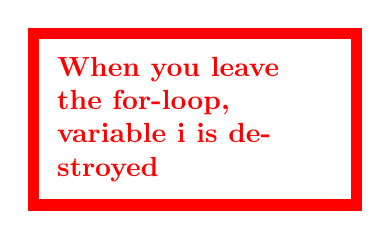
\begin{tikzpicture}
        \node[draw,minimum height=2cm,text width=3.5cm, line width=0.15cm, color=red, font=\normalsize\bfseries, inner sep=0.3cm] (b) at (-6.7,10.1) {When you leave the for-loop,\\variable i is destroyed};
\end{tikzpicture}
}

Note that the above simulation is only a \emph{\textbf{\underline{model}}}.
Furthermore, it does not explain how the computer knew that 4 $<$ 5 was true. And what does \lq\lq true'' really mean to a computer anyway? In fact, does a computer \lq\lq know'' what's a \lq\lq 4''  (as in four)??? For details like these you will have to take Assembly Language (CISS360) and Computer Architecture (CISS420).


\begin{ex}
There's one place where you can use
the pre-increment operator and another where you can use +=. Modify the
above code.
\end{ex}

\begin{ex}
Do the same trace with this program:
\begin{console}
int s = 10;
for (int i = 10; i < 14; i = i + 1)
{   
    s = s + i;
}
std::cout << s << std::endl;
\end{console}
\end{ex}
What is the output? Now run the program with your C++ compiler and
verify.

\begin{ex}
Do the same trace with this program:
\begin{console}
int s = 0;
for (int i = 3; i < 10; i += 2)
{   
    s = s + i;
}
std::cout << s << std::endl;
\end{console}
\end{ex}

What is the output? Now run the program with your C++ compiler and
verify.

\begin{ex}
Do the same trace with this program:
\begin{console}
int s = 0;
for (int i = 0; i < 10; i = i + 1);
    s = s + i;
std::cout << s << std::endl;
\end{console}
\end{ex}
What is the output (or is there an error)? Now run the program with your
C++ compiler and verify.

\newpage\EMPHASIZE{Using \texttt{for}-loop to compute sums}

Look at the following program:
\begin{console}
int sum = 0;
int i = 1;

sum = sum + i;
i = i + 1;

sum = sum + i;
i = i + 1;

sum = sum + i;
i = i + 1;

sum = sum + i;
i = i + 1;

sum = sum + i;
i = i + 1;

sum = sum + i;
i = i + 1;

sum = sum + i;
i = i + 1;

sum = sum + i;
i = i + 1;

sum = sum + i;
i = i + 1;

sum = sum + i;
i = i + 1;

std::cout << sum << std::endl;
\end{console}

OK. \ldots looks like a long program \ldots but most of it repeats.

Now look at this one:
\begin{console}
int sum = 0;
for (int i = 1; i <= 10; i = i + 1)
{   
    sum = sum + i;
}
std::cout << sum << std::endl;
\end{console}

Do you see that they do the same thing? Make sure you trace both
programs by hand and see that the actual computations are the same.

\begin{ex}
Modify the \texttt{i = i + 1} so that the plus
augmented operator is used. (Don't peek ahead!)
\end{ex}
\begin{ex}
You can get C++ to tell us what's
happening in the for-loop by pausing the loop like this:
\begin{console}[commandchars=\~\@\$]
int sum = 0;
for (int i = 1; i <= 3; i++)
{   
     ~textbf@char c;$
     ~textbf@std::cout << "enter a char to continue ...";$
     ~textbf@std::cin >> c;$

     sum = sum + i;
     ~textbf@std::cout << i << ' ' << sum << std::endl;$
}
std::cout << sum << std::endl;
\end{console}
\end{ex}

Make sure you try this. This is a \EMPHASIZE{very basic technique} for
slowing down a loop so that you can follow what's
happening and do \EMPHASIZE{debugging}.

\begin{ex}
 Rewrite the program to use an augmented operator.
(Yes, there's one other place where you can use an
augmented operator.)
\end{ex}

\begin{ex}
 Modify the above program to compute the sum of all
integers from 1 to 100. You want to remove the pause in the middle of
the program:
\begin{console}[commandchars=\~\@\$]
int sum = 0;
for (int i = 1; i <= 3; i++)
{   
    ~sout@char c;$
    ~sout@std::cout << "enter something to continue ...";$
    ~sout@std::cin >> c;$
    
    sum = sum + i;
    ~textbf@std::cout << i << ' ' << sum << std::endl;$
}
std::cout << sum << std::endl;
\end{console}
\end{ex}

\begin{ex}
Modify the above program to compute the sum of squares from $1^{2}$ to $5^{2}$. Verify your program by calculating this sum with a calculator. Modify your program to compute the sum of squares from $1^{2}$ to $100^{2}$. Of course the number is going to be really huge \ldots you do not want to check this one with your calculator!
\end{ex}

\begin{ex}
Modify the above program to compute the sum of reciprocals of squares from $1/1^{2}$ to $1/5^{2}$. (What type of values are you adding to \texttt{sum}? What should the type of \texttt{sum} be?) Verify your program by calculating this \texttt{sum} with a calculator. Modify your program to compute the sum of reciprocals of squares from $1/1^{2}$ to $1/100^{2}$. Compare to the previous exercise and note that the sum stabilizes quickly since the terms you're adding to the sum shrink very quickly. In this case we say that the sum \EMPHASIZE{converges}. You can try to modify your program to add up to $1/1000000^{2}$. You'll find that it won't change the sum much.
\end{ex}

\begin{ex}
Modify the above program to compute

\[1/1 + 1/2 + 1/3 + \ldots + 1/100\]

In this case, the sum seems to stabilize since each term you add to the
sum shrinks. However the sum is actually NOT stabilizing. It is actually
growing \ldots but very slowly. You can try to compute the sum up to
1/1000000.
\end{ex}

In general the computation of a sum using a loop looks like this:
\begin{flushleft}
\text{sum = 0}\\
\text{for i running from a, a+1, a+2, \ldots, b:}\\
\tab[1em]{\text{sum = sum + (some term)}}
\end{flushleft}
For instance:
\begin{flushleft}
\texttt{sum = 0;}\\
\texttt{for (int i = 1; i <= 100; ++i)}\\
\{
\tab[1em]{\texttt{sum += i;}}\\
\}
\end{flushleft}
In this case the term to add to \texttt{sum} is \texttt{i}. If you want to
sum squares you can do this:
\begin{flushleft}
\texttt{sum = 0;}\\
\texttt{for (int i = 1; i <= 100; ++i)}\\
\{\\
\tab[1em]{\texttt{sum += i * i;}}\\
\}\\
\end{flushleft}
or this:
\begin{flushleft}
\texttt{sum = 0;}\\
\texttt{for (int i = 1; i <= 100; ++i)}\\
\{\\
\tab[1em]{\texttt{int term = i * i;}}\\
\tab[1em]{\texttt{sum += term;}}\\
\}\\
\end{flushleft}
Of course for such cases, the term can be computed from \texttt{i}.
There's no reason why the term cannot be supplied by,
for instance, a user. Here's one that adds integers
specified by a user:
\begin{console}
int num_accts;
std::cout << "how many bank accounts do you have? ";
std::cin >> num_accts;

double sum = 0;
for (int i = 1; i <= num_accts; ++i)
{
        std::cout << "enter amt in bank acct #"
                  << i << "? $";
        double amt;
        std::cin >> amt;
        sum += amt;
        std::cout << "so far ... you have $"
                  << sum << std::endl;
}
std::cout << "total ... you have $"
          << sum << std::endl;
\end{console}
\begin{ex}
 Write a program that first asks a user how many
houses he/she has. Next the program asks the user for the number of
rooms in each house. Finally, the program prints the total number of
rooms he/she has for all the properties owned by the user.
\end{ex}
\begin{ex}
 Write a program that first asks a user how many
houses he/she has. Next the program asks the user for the number of
rooms in each house and the average square footage for the rooms in that
house. Finally, the program prints the total square footage of all the
rooms across all the properties owned by the user.
\end{ex}
\newpage\EMPHASIZE{Using for-loop to compute products}

\begin{ex}
Trace this by hand:
\begin{console}[commandchars=\~\@\$]
int product = 1;
for (int i = 1; i <= 5; i++)
{   
    product *= i;
    std::cout << i ~textbf@<< ' ' <<$ product << std::endl;
}
std::cout << product << std::endl;
\end{console}
\end{ex}

What is the output (or is there an error)? Now run the program with your
C++ compiler and verify.

By the way, the product of all positive integer from 1 to 5 (i.e.
1x2x3x4x5) is called the \EMPHASIZE{factorial} of 5. The factorial of 10 is
just
\begin{center}
1 x 2 x 3 x 4 x 5 x 6 x 7 x 8 x 9 x 10
\end{center}
In general, the factorial of n is such an important quantity that we
have a shorthand notation for it: The factorial of n is written n!. So
\begin{center}
10! = 1 x 2 x 3 x 4 x 5 x 6 x 7 x 8 x 9 x 10
\end{center}
Note that the factorial of 0 is defined to be 1.
\begin{center}
0! = 1
\end{center}
Study the above code. Do you see that it computes the factorial of 5?

The factorial appears in Computer Science, Math, Physics, Chemistry,
Finance, etc. So you bet it's important.

\begin{ex}
Compute by hand the factorial of n for n = 0, 1, 2, 3, 4, 5, 6. Use your calculator to verify your work. Using C++, compute the factorial of 10.
\end{ex}
\begin{ex}
 Why did I initialize \texttt{product} with \texttt{1} and
not \texttt{0}? What if you run this program instead?
\begin{console}
int product = 0;
for (int i = 1; i <= 5; i++)
{   
    product *= i;
    std::cout << i << ' ' << product << std::endl;
}
\end{console}
And what if I initialize the \texttt{product} to 2? (See why it has to be
initialized to \texttt{1} now?)
\end{ex}

\begin{ex}
Write a program that prompts the user for n and
prints the product of \texttt{\textbf{odd}} integers greater than 0 and
less than n.
\end{ex}

\begin{ex}
Write a program that prompts the user for n (an
integer value at least 0) and prints 2-to-the-power of n. For instance,
if the user enters 0, the program prints 1; if the user enters 3, the
program prints 8; if the user entered 10, the program prints 1024; Etc.
\end{ex}

\begin{ex}
Write a program that prompts the user for \texttt{x} (a
\texttt{double}) and then \texttt{n} (an \texttt{int} value at least \texttt{0})
and prints \texttt{x}-to-the-power of \texttt{n}. Check your program with
several cases, testing it either by hand or by using a calculator.
\end{ex}

\begin{ex}
Write a program that prompts the user for \texttt{x} (a \texttt{double}) and then \texttt{n} (an \texttt{int} value \underline{\textbf{\emph{which can be negative}}}) and prints \texttt{x}-to-the-power
of \texttt{n}. Check your program with several cases, testing it either by
hand or by using a calculator.
\end{ex}
\begin{ex}
Besides the factorial function n!,
there's another quantity that is extremely important in
Computer Science, Math, Physics, and you-name-it. It's
called the n-choose-r function. It's sometimes written
C(n,r). It depends on the factorial. Let n and r be positive integers
where r is at most n. Then n-choose-r is given by
\end{ex}
\begin{center}
n! / (r! (n - r)!)
\end{center}
n-choose-r is the total numbers of ways to choose r things from n
distinct things. For instance, suppose you are an IT manager and have a
team of 40 programmers, and you have to form a team of 5 software
engineers. The total numbers of ways to form this team is 40-choose-5,
i.e.,
\begin{center}
40! / (5! x (40 - 5)!) = 40! / (5! x 35!)
\end{center}
However 40! is too huge to compute. Use your program to compute
5-choose-2. Verify the correctness of your program by doing this
computation by hand. Here are 5 symbols:

\begin{center}
a, b, c, d, e
\end{center}
Write down all possible selections of 2 symbols. Let me begin for you:
\begin{align*}
\text{a, b}\\
\text{a, c}
\end{align*}

Note that the selection of a, b is considered the same as the selection of b, a. So do not include b, a. Likewise only include b, e and not e, b.

\newpage\EMPHASIZE{Using for-Loop to compute min/max}

Recall that if you have int variables a, b, c, d, and you want to
compute the minimum, you can do this (pseudocode only!):
\begin{console}
min = a
if b < min:
   min = b
if c < min:
   min = c
if d < min:
   min = d
\end{console}
In this case min is an integer variable. (Re-study your notes on the if
statement if you don't recall this!!!)

The idea of course works for doubles too. Of course the min variable
must be declared to be a double variable. Make sure you understand the
above!

The idea for the computation of the maximum is similar.

Now the above sure looks like a loop. If the values are not stored in
variables a, b, c, d but for instance is supplied by the user (so we
need to do std::cin), then we have a very compact way to compute the
minimum of 4 values supplied by the user. Instead of doing
\begin{console}
prompt user for a
min = a

prompt user for b
if b < min:
   min = b

prompt user for c
if c < min:
   min = c

prompt user for d
if d < min:
   min = d

print min
\end{console}
we can do this:

\begin{console}
prompt user for x
min = x

// 3 more values
for i = 0, 1, 2:
    prompt user for x
    if x < min:
       min = x
       
print min
\end{console}

(user inputs are all stored using x).

The C++ code is then:

\begin{console}
int x;
int min;

std::cin >> x;
min = x;

// 3 more values, so i = 0, 1, 2 works.
for (int i = 0; i < 3; i++)
{   
    std::cin >> x;
    if (x < min)
    {
        min = x;
    }
}
std::cout << min << std::endl; 
\end{console}
Not only that, this code can be EASILY modified to compute the minimum
of 10 values:

\begin{console}
int x;
int min;

std::cin >> x;
min = x;

// i = 0, 1, 2, 3, 4, 5, 6, 7, 8 --- 9 more values
for (int i = 0; i < 9; i++)
{   
    std::cin >> x;
    if (x < min)
    {
        min = x;
    }
}
std::cout << min << std::endl;
\end{console}

The old method without loops would take a lot more time to write!

Not only that, the above method works when you allow the user to specify
how many values the user wants to input!!

\begin{console}
int x;
int min;
int n; // number of values for the min computation

std::cin >> n;
std::cin >> x;
min = x;

for (int i = 0; i < n - 1; i++)
{   
    std::cin >> x;
    if (x < min)
    {
        min = x;
    }
}

std::cout << min << std::endl;
\end{console}

As you can see, the loop is indispensable!!!
\begin{ex}
Write a program that prompts the user for n and then
prompts the user for n double values and then prints the maximum of the
values enters by the user.
\end{ex}
\begin{ex}
 Write a program that prompt the user for n and then
prompts the user for n double values and then prints the minimum of the
\textbf{absolute values} of the values entered by the user. Recall from
MATH104 that the absolute value of x is just x without the negative
sign. So for instance
\end{ex}
\begin{center}
$|42| = 42$

$|-24| = 24$
\end{center}

The absolute value functions were mentioned in the set of notes on
doubles. For your convenience, here's the information
again. For C++, if you need the absolute value of an integer value this
is how yo do it:
\begin{console}
#include <iostream>
#include <cstdlib>

int main()
{   
    int x = 42, y = -24;
    std::cout << abs(42) << '\n';
    std::cout << abs(-42)<< '\n'; 
    std::cout << abs(x) << '\n'; 
    std::cout << abs(y) << '\n';
    return 0;
}
\end{console}

If you need to compute the absolute value of doubles or floats you do
this:
\begin{console}
#include <iostream>
#include <cmath>
int main()
{   
    int x = 4.2, y = -2.4;
    std::cout << fabs(42) << '\n';
    std::cout << fabs(-42)<< '\n'; 
    std::cout << fabs(x) << '\n'; 
    std::cout << fabs(y) << '\n';
}
return 0;
\end{console}


\newpage\EMPHASIZE{The boolean condition}

Here's one of our first few programs:
\begin{console}
std::cout << "entering the for-loop ...\n";
for (int i = 10; i > 0; i--)
{   
    std::cout << "entered the block ...\n";
    std::cout << "i: " << i;
    std::cout << "exiting the block ...\n";
}
std::cout << "done with the for-loop ...\n";
\end{console}

Look at this boolean expression:
\begin{console}[commandchars=\~\@\$]
std::cout << "entering the for-loop ...\n";
for (int i = 10; ~EMPHASIZE@i > 0$; i--)
{   
    std::cout << "entered the block ...\n";
    std::cout << "i: " << i;
    std::cout << "exiting the block ...\n";
}
std::cout << "done with the for-loop ...\n";
\end{console}
One of the most common misconceptions about the for-loop (and actually
applies to all loops) is that many first-time programmers think that if
the boolean expression
\begin{center}
\EMPHASIZE{i $>$ 0}
\end{center}
is false at \EMPHASIZE{any point} in the loop, you will break you out of
the for-loop immediately. That's \EMPHASIZE{NOT TRUE}. Look
at the picture on page 12 again. The check on whether to break out of
the loop occurs at a specific point. If I do this instead:
\begin{console}[commandchars=\~\@\$]
std::cout << "entering the for-loop ...\n";
for (int i = 10; ~EMPHASIZE@i > 0$; i--)
{   
    std::cout << "entered the block ...\n";
    std::cout << "i: " << i;
    ~EMPHASIZE@i = 0;$
    std::cout << "exiting the block ...\n";
}
std::cout << "done with the for-loop ...\n";
\end{console}


The program would still execute the last statement in the body of the
for-loop:
\begin{center}
\texttt{std::cout << "exiting the block ...\ n";}
\end{center}
because the boolean check comes after this print statement.
\begin{center}
\EMPHASIZE{MAKE SURE YOU REMEMBER THAT!}
\end{center}

\newpage\EMPHASIZE{Generating Equally Spaced Points on a Line}

In the next two sections, we will generate points in a range which are
equally spaced. This is what I mean:

Suppose I tell you that I want 5 equally spaced points on the interval [0, 4] that includes the end points 0 and 4. You would say:
\begin{center}
0, 1, 2, 3, 4
\end{center}
There are 5 values. They are equally spaced: consecutive values differ
by 1. The first value 0 is the left endpoint of [0, 4] and the last
value 4 is the right endpoint of [0, 4].

What if I ask you for 3 equally spaced points on [0, 4] including
both end points? Well this means that you want 3 values, say we call
them
\begin{center}
x0, x1, x2
\end{center}
where x0 is 0 and x2 is 4. What about x1? x1 is right in the middle. So
it must be
\begin{center}
x1 = (x2 -- x1) / 2 = 2
\end{center}
So the values are
\begin{center}
0, 2, 4
\end{center}
Great! Done!

What if I ask you for 4 equally points in [0, 4]?
Let's call then
\begin{center}
x0, x1, x2, x3
\end{center}
Of course
\begin{center}
x0 = 0
x3 = 4
\end{center}
What about x1 and x2? Well since they are equally spaced,
let's say the gap between x0 and x1 is d. Since the
points are equally spaced, the gap is of course also the gap between
x1,x2 and also x2,x3. There are altogether 3 gaps and they add up to 4.
So
\begin{center}
d = 4/3
\end{center}
(as a real number, i.e., double. The above is math, not C++) In other
words:
\begin{center}
d = 1.3333.... (up to 4 decimal places)
\end{center}
This mean that
\begin{align*}
\text{x0 = 0}\\
\text{x1 = 0 + d = 1.3333....}\\
\text{x2 = x1 + d = 2.6666...}\\
\text{x3 = x2 + d = 4}\\
\end{align*}
What if I want \EMPHASIZE{7} points in the same interval? Say the points
are
\begin{center}
x0, x1, x2, x3, x4, x5, x6
\end{center}
There are \EMPHASIZE{6} gaps. Call the gap d. The gaps add up to 4.
Therefore
\begin{center}
6d = 4
\end{center}
i.e.,
\begin{center}
d = 4/6 = 0.6666...
\end{center}
and the values of the points are
\begin{align*}
\text{x0 = 0}\\
\text{x1 = x0 + d}\\
\text{x2 = x1 + d}\\
\text{x3 = x2 + d}\\
\text{x4 = x3 + d}\\
\text{x5 = x4 + d}\\
\text{x6 = x5 + d}\\
\end{align*}

Writing this as a C++ program I get
\begin{console}
double x = 0;
double d = double(4) / 6
for (int i = 0; i < 7; ++i)
{   
    std::cout << x << '\n';
    x += d
}
\end{console}
Run this and check that you do get 7 points which are equally spaced.

\begin{ex}
 Modify the following code to generate equally spaced
points in [0, 4] if the number of points is n.
\begin{console}
int n;
std::cin >> n;
double x = 0;
double d = double(4) / 6;
for (int i = 0; i < 7; ++i)
{   
    std::cout << x << '\n';
    x += d
}
\end{console}
Test your program for different values of \texttt{n}.
\end{ex}

\begin{ex}
If the interval is not [0, 4] but [0, b] and the number of points is n, then modify the following code as appropriate:
\begin{console}
int n = 0;
double b = 0.0;
std::cin >> b;
std::cin >> n;

double x = 0;
double d = double(4) / 6;
for (int i = 0; i < 7; ++i)
{   
    std::cout << x << '\n';
    x += d
}
\end{console}
Test your code thoroughly.
\end{ex}

\begin{ex}
If the interval is [a, b] and the number of points is n, then modify the following code as appropriate:
\begin{console}
int n = 0;
double a = 0.0, b = 0.0;
std::cin >> a >> b;
std::cin >> n;

double x = 0;
double d = double(4) / 6;
for (int i = 0; i < 7; ++i)
{   
    std::cout << x << '\n';
    x += d
}
\end{console}
Test your code thoroughly. [Hint: Move the interval so that the left
endpoint is 0. The interval becomes [0, b -- a]. Get the points
using the previous exercise. Now move the points back to [a, b].
\end{ex}
WARNING \ldots INCOMING SPOILER!!!

Here's the answer to the above. If you are generating n
equally spaced points in the interval a, b] (and the left and right
end points are included), the code is
\begin{console}
double x = a;
double d = double(b - a) / (n - 1);
for (int i = 0; i < n; ++i)
{   
    std::cout << x << '\n';
    x += d
}
\end{console}

Note that because of rounding errors (remember that doubles and floats
are not exact!), the last point might not be exactly the value b. You
can stop the for-loop earlier and manually use b for the last point:
\begin{console}
double x = a;
double d = double(b - a) / (n - 1);
for (int i = 0; i < n - 1; ++i)
{   
    std::cout << x << '\n';
    x += d;
}

x = b;
std::cout << x << '\n';
\end{console}

In the next couple of sections, we will be using these equally spaced
points to do some computations. So in the general case, the code will
look something like this:
\begin{console}[commandchars=\~\@\$]
double x = a;
double d = double(b - a) / (n - 1);
for (int i = 0; i < n - 1; ++i)
{
~textbf@{... do something with x ...}$
x += d;
}
x = b;
~textbf@... do something with x ...$
\end{console}

\newpage\EMPHASIZE{Sums again: Area computation}

I'm going to use the \texttt{for}-loop to compute a certain sum.
This time it's going to be the area under a curve. The computation of areas is extremely important in many areas of science.

The idea is actually very simple: you need to know how to compute the area of rectangles and you need to be able to add lots of these areas.

The idea is pretty simple and illustrates the power of being able to do perform repetitions quickly.

First you draw the graph of the function, for example, y = f(x) = x*x, the standard parabola):

%%\includegraphics[width=4.5in,height=2.7736in]{Pictures/10000000000002B3000001AAC5D1A577C30A5997.png}

Suppose you want to compute the area under this curve and above the
x-axis and from x = 2 to x = 7:

%\includegraphics[width=4.5in,height=2.5165in]{Pictures/10000000000002CD000001911B1B47C442016F8D.png}

You can make an approximation by computing the areas of the rectangles
with
\begin{align*}
\text{x=2 to x=3 with height f(2)}\\
\text{x=3 to x=4 with height f(3)}\\
\text{x=4 to x=5 with height f(4)}\\
\text{x=5 to x=6 with height f(5)}\\
\text{x=6 to x=7 with height f(6)}\\
\end{align*}
There are altogether 5 rectangles. Draw these rectangles into the graph
above.

%\includegraphics[width=4.5in,height=2.5362in]{Pictures/10000000000002CB00000193C61596A9DE7C6C44.png}

Note that for each rectangle, the base has width 1. Also, for each
rectangle, I am using the left endpoint on the width to determine the
height. The areas of these rectangles is smaller than the area under the
parabola from x = 2 to 2 = 7.

\begin{ex}
Write a for-loop to compute the sum of the above
rectangles. Write down the sum of areas. We'll need it
for comparison later.
\end{ex}
Now we \lq\lq move'' the sum of areas of our rectangles towards the parabola
in the following way: we will use \textbf{more} rectangles. Previously the
base of the rectangles had a width of 1. Now I'm going
to use rectangles with base of length 0.5. Altogether we now have 10
rectangles:
\begin{align*}
\text{x=2.0 to x=2.5 with height f(2.0)}\\
\text{x=2.5 to x=3.0 with height f(2.5)}\\
\text{x=3.0 to x=3.5 with height f(3.0)}\\
\text{x=3.5 to x=4.0 with height f(3.5)}\\
\text{x=4.0 to x=4.5 with height f(4.0)}\\
\text{x=4.5 to x=5.0 with height f(4.5)}\\
\text{x=5.0 to x=5.5 with height f(5.0)}\\
\text{x=5.5 to x=6.0 with height f(5.5)}\\
\text{x=6.0 to x=6.5 with height f(6.0)}\\
\text{x=6.5 to x=7.0 with height f(6.5)}\\
\end{align*}
Draw these 10 rectangles into the above graph.

%\includegraphics[width=4.5in,height=2.5492in]{Pictures/10000000000002C9000001940CA977BFEBA1D44B.png}

Do you see that the total area of these rectangles are closer to the
actual area under the parabola than the one from our first
approximation?

Do you see that, intuitively, the total area of the rectangles gets
closer and closer to the area under the parabola from x = 2 to x = 7 as
the number of rectangles used increases? Here's the case
where the length of the base of the rectangles is 0.25:

%\includegraphics[width=4.5in,height=2.5181in]{Pictures/10000000000002C90000018F19E7A9D9A73C9FA9.png}
and here's the case where the length is 0.125

%\includegraphics[width=4.4272in,height=2.139in]{Pictures/10000000000002CA00000191D2EF8AEA529C84AC.png}

Using the code that computes equally spaced point, the sum of the areas
of these rectangles can thus be computed as follows:
\begin{console}
double a = 2;
double b = 7;
int n = 11; // 10 rects mean 11 points
double sum = 0;
double x = 0;
double d = double(b - a) / (n - 1);
for (int i = 0; i < n - 1; ++i)
{   
    sum += d * (x * x);
    x += d;
}

// Why do we NOT need to execute the following?
// x = b;
// sum += d * (x * x);
\end{console}
\begin{ex}
Compute area when 20 rectangles are used.
\end{ex}
\begin{ex}
Now do the same where you use 100 rectangles.
\end{ex}

Now write a program that prompts the user for the number of rectangles!
Say we call this variable n. Run the program with n = 1000 rectangles!!!
You bet the value computed by your program is extremely close to the
real area of the parabola. Of course you wouldn't add
the areas of 1000 rectangles by hand -- it would take too long!
That's what a program is for -- if you know C++!!!

\begin{ex}
If you know some Calculus 1, you know that the area
under the parabola from x = 2 to x = 7 is in fact exactly
\[(1 / 3)(7 * 7 * 7 -- 2 * 2 * 2)\]

Use your calculator (or C++) to compute this value and compare against
the value obtained by your program with n = 1000 rectangles.
\end{ex}

\begin{ex}
The above prompts the user for n, the number of
rectangles to use for the area computation using a for-loop. Write a
nested for-loop where the outer for-loop supplies values of n running
from 1000 to 1000000 by increments of 1000. The pseudocode looks like
this:
\begin{align*}
\text{for n = 1000, 2000, 3000, \ldots, 1000000:}\\
\tab[3em]{\text{compute and print the area using n rectangles}}
\end{align*}
\end{ex}

\begin{ex}
 Modify the above program so that instead of computing
the area under the parabola from x = 2 to x = 7, the program prompts the
user for a, b, n and computes the area under the parabola from x = a to
x = b using n rectangles.
\end{ex}

\begin{ex}
 What is the area under the curve y = x*x*x from x=0
to x=10?
\end{ex}

The computation of areas under a curve is important. For instance in
Physics, the work done by a force F is the area under the
force-displacement graph where you plot the force acting on an object
and the displacement of the object. By Newton's law of
universal gravitation, we know the gravitational force between two
objects which are apart from each other at a fixed distance. So if a
rocket wants to move away from earth, you can compute the work done
moving the rocket to a distance from the surface of earth to a far away
point in space. Knowing the work to be done moving the rocket from earth
through a required distance, you can then compute the amount of chemical
fuel that is needed to combust in order to convert the chemical energy
into required work done. Of course there are many other applications of
the computation of areas.

\newpage\EMPHASIZE{Root finding: An inefficient method}

Another very common problem in Math and Sciences is finding solution(s)
to an equation such as finding solutions to quadratic equations:

\[2 * x * x + 4 * x - 3 = 0\]

This is easy since we have the quadratic equation formula. But this is
highly non-trivial if the equation is more complex such as a degree 5
equation:

\[2 * x * x * x * x * x + 4 * x * x - 3 * x + 10 = 0\]

or even one with trigonometric, logartihmic, and/or exponential
functions!!!

For instance, what if I want to find a solution to

\[3 * x * x - 10 * x * sin(x) - 500 = 0\]

in the range [0, 20]? You don't recall a solution to
such an equation from your math classes right?!?

Since we don't have a formula to use, we just have to
plot the graph and visually see where the function touches the x-axis.
In the same way, we can compute the values of the above expression

\[3 * x * x - 10 * x * sin(x) - 500\]

for many many many many many values in the range [0, 20] and see
which value of x will give a value of

\[3 * x * x - 10 * x * sin(x) - 500\]

that is very close to 0. For instance we can test 1,000,000 values in
the range [0,20]. If we do this by hand, we would go crazy. But
\ldots

We know C++!!!!

All we need to do is to run a for-loop of 1,000,000 values in the range
[0,20] and find the value of x that will get use as close as
possible to the y-axis. Close to the y-axis means

\[|f(x)|\]

is close to zero. In other words, if you're finding the
point closest to the y-axis it means that you need to find the smallest
$|f(x)|$ for the 1,000,000 x values in the range.

\begin{ex}
Using a \texttt{for}-loop, find a value for x from 1 to 5 such
that x sin(x) + 1 is as close as possible to the x-axis.
\end{ex}
\newpage\EMPHASIZE{Maximum and minimum of functions}

Using the idea of generating lots and lots of equally spaced points on
an interval, you can very quickly compute the approximate maximum and
minimum of functions. Note that the max or min is only an approximation
since your points might miss the actual maximum and minimum.

\begin{ex}
Write a program to compute and print the maximum
value of the sine function on the interval [0, 10] using 1,000,000
equally spaced points. The sine function is already mentioned in the
notes on floating point values.
\end{ex}

\begin{ex}
Modify the above program so that it prints the value
of x where the maximum occurs.
\end{ex}

\begin{ex}
Compute and print the maximum and minimum value of
the function
\begin{center}
f(x) = x sin(x)
\end{center}
on the interval [0, 20] using 1,000,000 points. When you're done, modify the program to also print the x value where the maximum and minimum occurs.
\end{ex}
